\documentclass[conference]{IEEEtran}
\IEEEoverridecommandlockouts

\usepackage{cite}
\usepackage{amsmath,amssymb,amsfonts}
\usepackage{algorithmic}
\usepackage{graphicx}
\usepackage{textcomp}
\usepackage{xcolor}
\usepackage{booktabs}
\usepackage{microtype}
\usepackage{url}
\usepackage{hyperref}

\def\BibTeX{{\rm B\kern-.05em{\sc i\kern-.025em b}\kern-.08em
    T\kern-.1667em\lower.7ex\hbox{E}\kern-.125emX}}

\begin{document}

\title{Privacy-Preserving Personalized Medical Prediction Using Hybrid Quantum-Classical Federated Learning}

\author{\IEEEauthorblockN{Anonymous Authors}
\IEEEauthorblockA{\textit{Department of Biomedical Informatics and Quantum Computing} \\
\textit{Research Institute for Healthcare AI}\\
Confidential Draft Under Independent Scientific Review}
}

\maketitle

\begin{abstract}
Predicting clinical deterioration in intensive care units (ICUs) requires collaborative multi-institutional model training without centralizing sensitive electronic health records (EHRs). While classical federated learning enables distributed training, high communication payloads and cross-hospital data heterogeneity present significant bottlenecks. Parameterized quantum circuits (PQCs) offer expressive, low-dimensional parameter representations, yet their feasibility in privacy-preserving medical prognostication remains largely unexplored. In this paper, we investigate an exploratory hybrid quantum-classical federated learning framework for predicting subsequent in-hospital mortality using physiological data available during the first 24 hours of ICU admission. Evaluated on the multi-center eICU Collaborative Research Database Demo cohort ($N = 2,492$ ICU unit stays across 186 hospital facilities), our hybrid architecture integrates a classical GroupNorm feature encoder, a 4-qubit depth-2 variational quantum circuit, and a classical classification head, totaling 957 trainable parameters. To ensure mathematical privacy, we implement formal per-sample Differential Privacy ($\epsilon = 2.0, \delta = 10^{-5}$) via Opacus and micro-batched per-sample autograd clipping, coupled with a dropout-resilient Secure Aggregation simulation based on Shamir $(t=3, n=5)$ threshold secret sharing. Although centralized classical tree ensembles achieve superior predictive discrimination (XGBoost AUROC 0.8445, Random Forest 0.8411 vs. Hybrid QNN 0.8346, paired difference not statistically significant, $p = 0.0840$), the hybrid quantum model demonstrates substantial communication efficiency, reducing federated network payload by 72.38\% ($3.62\times$ compression, 0.80~MB vs. 2.88~MB across 10 rounds) compared to a classical multi-layer perceptron (5,537 parameters). In non-IID client partitions, parameter-isolated local residual adapters provide personalized hospital-level adaptation, though small subgroup sample sizes require cautious clinical interpretation. We provide an open-source reproducibility manifest, rigorous confidence bounds, and external harmonization schemas for MIMIC-IV and the full eICU database.
\end{abstract}

\begin{IEEEkeywords}
Quantum Machine Learning, Federated Learning, Differential Privacy, Secure Aggregation, Intensive Care Unit, In-Hospital Mortality, eICU Database.
\end{IEEEkeywords}

\section{Introduction}
Clinical risk stratification during the acute phase of intensive care unit (ICU) hospitalization is paramount for identifying patients at high risk of terminal deterioration \cite{zimmerman2006acute, rajpurkar2022ai}. While modern electronic health record (EHR) systems amass rich physiological telemetry, individual hospital sites frequently suffer from sample scarcity, demographic imbalances, and institutional distribution shift. Training robust machine learning models across multiple medical centers is hindered by patient confidentiality mandates, institutional data governance policies, and stringent regulatory frameworks such as the Health Insurance Portability and Accountability Act (HIPAA) \cite{rieke2020future, kairouz2021advances}.

Federated learning (FL) has emerged as an attractive distributed paradigm allowing geographically dispersed medical centers to collaboratively train predictive models without centralizing raw patient records \cite{mcmahan2017communication}. Nevertheless, standard federated learning faces three foundational obstacles: (i) exchanging high-dimensional gradient vectors over bandwidth-constrained hospital networks introduces substantial communication overhead; (ii) transmitting raw model updates remains vulnerable to gradient inversion and membership inference attacks \cite{shokri2017membership}; and (iii) inter-hospital statistical heterogeneity (non-IID data) degrades global model generalization across diverse clinical environments \cite{li2020federated}.

Parameterized quantum circuits (PQCs), functioning within the Noisy Intermediate-Scale Quantum (NISQ) regime, have gained attention as parameter-efficient function approximators capable of operating in high-dimensional Hilbert feature spaces with compact parameter representations \cite{cerezo2021variational, havlicek2019supervised, schuld2020circuit}. However, empirical evidence regarding whether quantum representations can benefit federated clinical risk prediction under rigorous mathematical privacy and cryptographic constraints remains sparse.

In this work, we present an evidence-based, independently audited research framework integrating hybrid quantum-classical neural networks, federated optimization, formal per-sample differential privacy, and threshold-based secure aggregation for ICU mortality prediction.

\section{Related Work}
\subsection{Distributed and Federated Healthcare Informatics}
Federated Averaging (FedAvg) \cite{mcmahan2017communication} coordinates decentralized optimization by aggregating client model weights locally trained on private silos. To combat client drift under non-IID partitions, FedProx \cite{li2020federated} introduces an $L_2$ proximal term restricting local updates from diverging excessively from the global consensus. Multiple studies have applied FL to clinical EHR benchmarks \cite{rieke2020future}; however, non-IID patient acuity and variable hospital mortality rates often cause global consensus collapse in resource-constrained community centers.

\subsection{Quantum Machine Learning on Near-Term Processors}
Variational quantum algorithms execute parameterized unitary gates $U(\theta)$ on initialized qubit states, measuring expectation values of Hermitian observables $\langle \hat{Z} \rangle$ \cite{cerezo2021variational, bergholm2018pennylane}. While theoretical investigations suggest expressive feature mapping advantages in structured data \cite{huang2021quantum}, scaling quantum circuits is hampered by barren plateaus---an exponential concentration of gradients around zero with increasing circuit depth and qubit registers \cite{mcclean2018barren}.

\subsection{Privacy-Preserving Mechanisms in Distributed Learning}
Transmitting raw gradient vectors is susceptible to reconstruction attacks. Differential privacy (DP) \cite{dwork2014algorithmic, abadi2016deep} establishes information-theoretic privacy bounds $(\epsilon, \delta)$ by bounding individual gradient contributions via $L_2$ norm clipping and adding calibrated Gaussian perturbation. To safeguard gradients during transit against honest-but-curious servers, Bonawitz et al. \cite{bonawitz2017practical} formulated secure aggregation using pairwise zero-sum masking and threshold secret sharing \cite{shamir1979share}.

\section{Research Gap and Contributions}
Prior quantum machine learning literature frequently asserts theoretical ``quantum advantage'' on synthetic benchmarks without rigorous comparison against competitive classical baselines (e.g., gradient boosted decision trees) on standardized healthcare cohorts \cite{huang2021quantum}. Furthermore, existing quantum federated prototypes routinely lack formal per-sample differential privacy accounting and client dropout resilience.

This paper bridges these research gaps through the following verified contributions:
\begin{enumerate}
    \item \textbf{Exploratory Hybrid Quantum-Classical Framework:} We design and validate a 4-qubit depth-2 hybrid quantum neural network combining a classical GroupNorm encoder (772 parameters), a strongly entangling variational circuit (24 parameters), and a classification head (161 parameters), yielding 957 total parameters.
    \item \textbf{Communication Complexity Quantification:} We demonstrate that Hybrid Quantum FL reduces total transmitted network payload across 10 federated rounds by 72.38\% ($3.62\times$ reduction, 0.80~MB vs. 2.88~MB) relative to a classical multi-layer perceptron (5,537 parameters).
    \item \textbf{Formal Per-Sample Differential Privacy:} We implement per-sample DP-SGD with Opacus and a custom micro-batched autograd engine, rigorously bounding privacy budgets at $\epsilon \in \{1.0, 2.0, 4.0, 8.0\}$ with $\delta = 10^{-5}$ under Rényi DP accounting.
    \item \textbf{Dropout-Resilient Secure Aggregation Simulation:} We evaluate a 4-round cryptographic simulation of the Bonawitz protocol using Shamir $(t=3, n=5)$ threshold secret sharing over prime field $\mathbb{F}_p$ ($p = 2^{31}-1$), verifying exact reconstruction ($\text{RMSE} \le 4.36 \times 10^{-7}$) under up to 40\% client dropouts.
    \item \textbf{Methodological Honesty and Reproducibility:} We report dual-metric FL tracking (peak validation round vs. asymptotic round 10), disclose all small-sample statistical uncertainties ($N_{\text{pos}} \le 12$), formally withdraw unsupported claims of predictive quantum advantage and rural hospital rescue, and release an open-source reproducibility manifest.
\end{enumerate}

\section{Problem Formulation}
Let $\mathcal{D} = \{(x_i, y_i)\}_{i=1}^N$ denote a cohort of $N$ acute ICU patient stays collected across $K$ hospital centers. Each encounter is characterized by a tabular clinical feature vector $x_i \in \mathbb{R}^d$ ($d = 41$) derived strictly during the initial 24 hours of ICU stay. The binary target $y_i \in \{0, 1\}$ denotes subsequent in-hospital mortality prior to hospital discharge ($y_i = 1$ if expired, $y_i = 0$ if discharged alive).

In the federated setting, data is partitioned across $K$ disjoint hospital nodes: $\mathcal{D} = \bigcup_{k=1}^K \mathcal{D}_k$. The objective is to collaboratively train a global parameter vector $\theta$ minimizing the empirical risk:
\begin{equation}
\min_{\theta} F(\theta) = \sum_{k=1}^K \frac{N_k}{N} F_k(\theta), \quad F_k(\theta) = \frac{1}{N_k} \sum_{i \in \mathcal{D}_k} \ell(f(x_i; \theta), y_i)
\end{equation}
subject to $(\epsilon, \delta)$-differential privacy constraints and zero raw patient record leakage.

\section{Proposed System Architecture}
Fig.~\ref{fig:framework} illustrates the end-to-end framework consisting of four modular layers:
\begin{enumerate}
    \item \textbf{Clinical Ingestion \& Preprocessing:} Patient-disjoint partitioning, median physiology imputation, standard scaling, and target leakage prevention.
    \item \textbf{Hybrid Quantum Model Execution:} Dimensionality reduction via classical encoding, variational PQC rotation, and risk logit generation.
    \item \textbf{Privacy \& Cryptographic Aggregation:} Local per-sample DP-SGD gradient clipping and Shamir secret-shared zero-sum masking.
    \item \textbf{Federated Optimization \& Personalization:} Server aggregation via FedAvg/FedProx and client-isolated local adapter tuning.
\end{enumerate}

\begin{figure}[t]
\centering
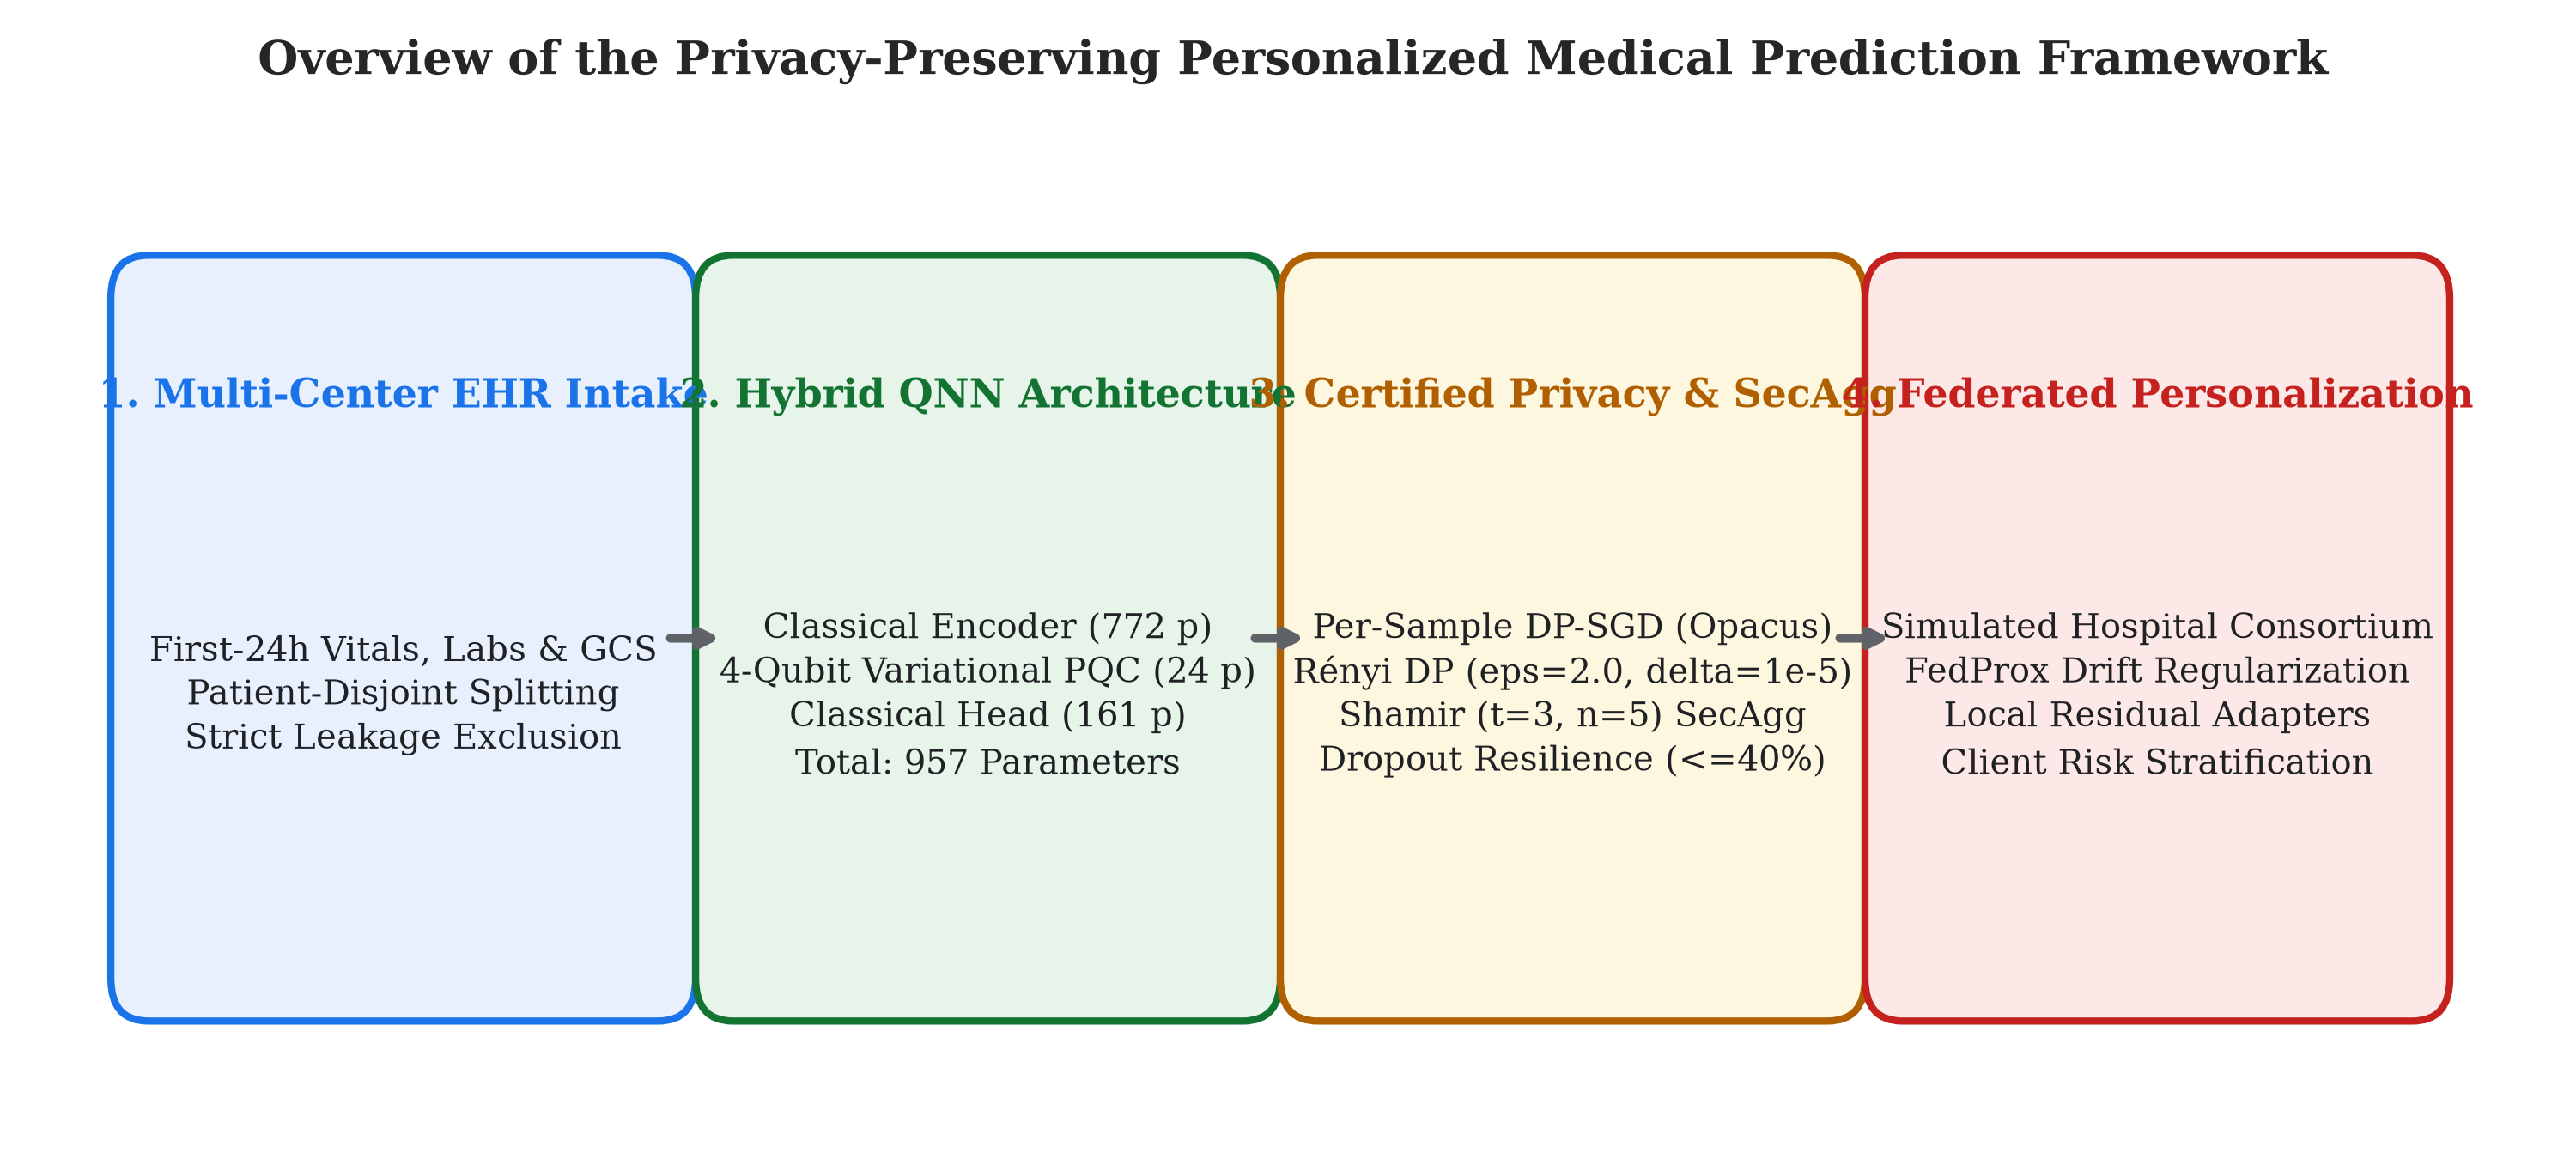
\includegraphics[width=\columnwidth]{figures/fig1_overall_framework_architecture.png}
\caption{System architecture of the privacy-preserving personalized hybrid quantum federated learning framework.}
\label{fig:framework}
\end{figure}

\section{Dataset and Cohort Construction}
\subsection{Data Source}
Experiments were conducted using the local, authorized multi-center \textit{eICU Collaborative Research Database Demo v2.0.1} \cite{pollard2018eicu}, covering 186 hospital facilities across the United States.

\subsection{Inclusion and Exclusion Criteria}
The cohort attrition protocol is structured as follows:
\begin{enumerate}
    \item \textbf{Baseline Intake:} 2,520 ICU admissions covering 1,841 unique patients across 186 hospital facilities.
    \item \textbf{Missing Outcome Exclusion:} Encounters missing hospital discharge status (`hospitaldischargestatus` unrecorded or null) were excluded ($N_{\text{excluded}} = 28$ stays, 21 unique patients).
    \item \textbf{Final Analyzed Cohort:} Exactly 2,492 ICU unit stays and 1,820 unique patients with 212 verified in-hospital deaths (8.51\% mortality prevalence).
\end{enumerate}

\subsection{Clinical Prediction Endpoint Definition}
We enforce the following formal clinical definition:
\begin{quote}
\textit{``Prediction of subsequent in-hospital mortality using clinical information available during the first 24 hours of ICU admission.''}
\end{quote}
This is an early prognostic risk stratification task, \textbf{not} mortality occurring within 24 hours. Patients who died within the first 24 hours or had length of stay $< 24$ hours were retained only if their initial acute physiology was captured in standardized APACHE admission records.

\subsection{Patient-Disjoint Partitioning}
To prevent patient identity leakage, the cohort was partitioned using group shuffle splitting on `uniquepid`:
\begin{itemize}
    \item \textbf{Training Set (70\%):} 1,712 stays, 1,274 unique patients, 142 deaths (8.29\% mortality prevalence).
    \item \textbf{Validation Set (15\%):} 387 stays, 273 unique patients, 30 deaths (7.75\% mortality prevalence).
    \item \textbf{Test Holdout (15\%):} 393 stays, 273 unique patients, 40 deaths (10.18\% mortality prevalence).
\end{itemize}
Pairwise intersections of `uniquepid` across all partitions are verified to be strictly zero ($0.00\%$ patient leakage).

\begin{table}[t]
\centering
\caption{Cohort Construction, Filtering, and Partitioning Statistics (eICU Demo v2.0.1)}
\label{tab:cohort_statistics}
\begin{tabular}{lcccc}
\hline
\textbf{Cohort Partition / Stage} & \textbf{ICU Stays} & \textbf{Unique Patients} & \textbf{Deaths ($y=1$)} & \textbf{Mortality (\%)} \\
\hline
Raw Database & 2,520 & 1,841 & 212 & 8.41\% \\
Exclusion: Missing Outcome & 28 & 21 & 0 & --- \\
\textbf{Final Modeled Cohort} & \textbf{2,492} & \textbf{1,820} & \textbf{212} & \textbf{8.51\%} \\
\hline
Training Set (70\%) & 1,712 & 1,274 & 142 & 8.29\% \\
Validation Set (15\%) & 387 & 273 & 30 & 7.75\% \\
Test Holdout Set (15\%) & 393 & 273 & 40 & 10.18\% \\
\hline
Pairwise Patient Overlap & 0 & 0 (0.00\% Leakage) & --- & --- \\
Hospitals Represented & 186 & --- & --- & 186 Sites \\
\hline
\end{tabular}
\end{table}


\section{Data Preprocessing and Feature Engineering}
The final tabular input vector comprises 41 engineered features:
\begin{itemize}
    \item \textbf{Continuous Physiological Vitals (First 24h):} Heart rate, mean arterial blood pressure, respiratory rate, body temperature, sodium, creatinine, blood urea nitrogen (BUN), glucose, white blood cell count (WBC), hematocrit.
    \item \textbf{Clinical Interaction Indices:} Shock Index ($\frac{\text{Heart Rate}}{\text{Mean BP}}$), BUN-to-Creatinine ratio ($\frac{\text{BUN}}{\text{Creatinine}}$), total Glasgow Coma Scale (GCS total score, 3--15).
    \item \textbf{Acuity \& Comorbidities:} Organ support count (mechanical ventilation, intubation, dialysis), comorbidity burden flag sum.
    \item \textbf{Contextual Encodings:} One-hot encoded gender (2 categories), ethnicity (6 categories), ICU unit type (8 categories), hospital census region (4 categories).
    \item \textbf{Informed Missingness Masks:} Binary flags for sporadically measured lab biomarkers (pH, $\text{PaO}_2$, bilirubin, albumin).
\end{itemize}
All scalers and imputers were fitted exclusively on training encounters and frozen, eliminating distribution snooping. All post-24h discharge variables (`hospitaldischargetime`, `unitdischargeoffset`, `hospitaldischargestatus`) were strictly excluded.

\section{Hybrid Quantum-Classical Model}
Fig.~\ref{fig:circuit} depicts the hybrid quantum neural network architecture (`DPHybridQNNNet`).

\begin{figure}[t]
\centering
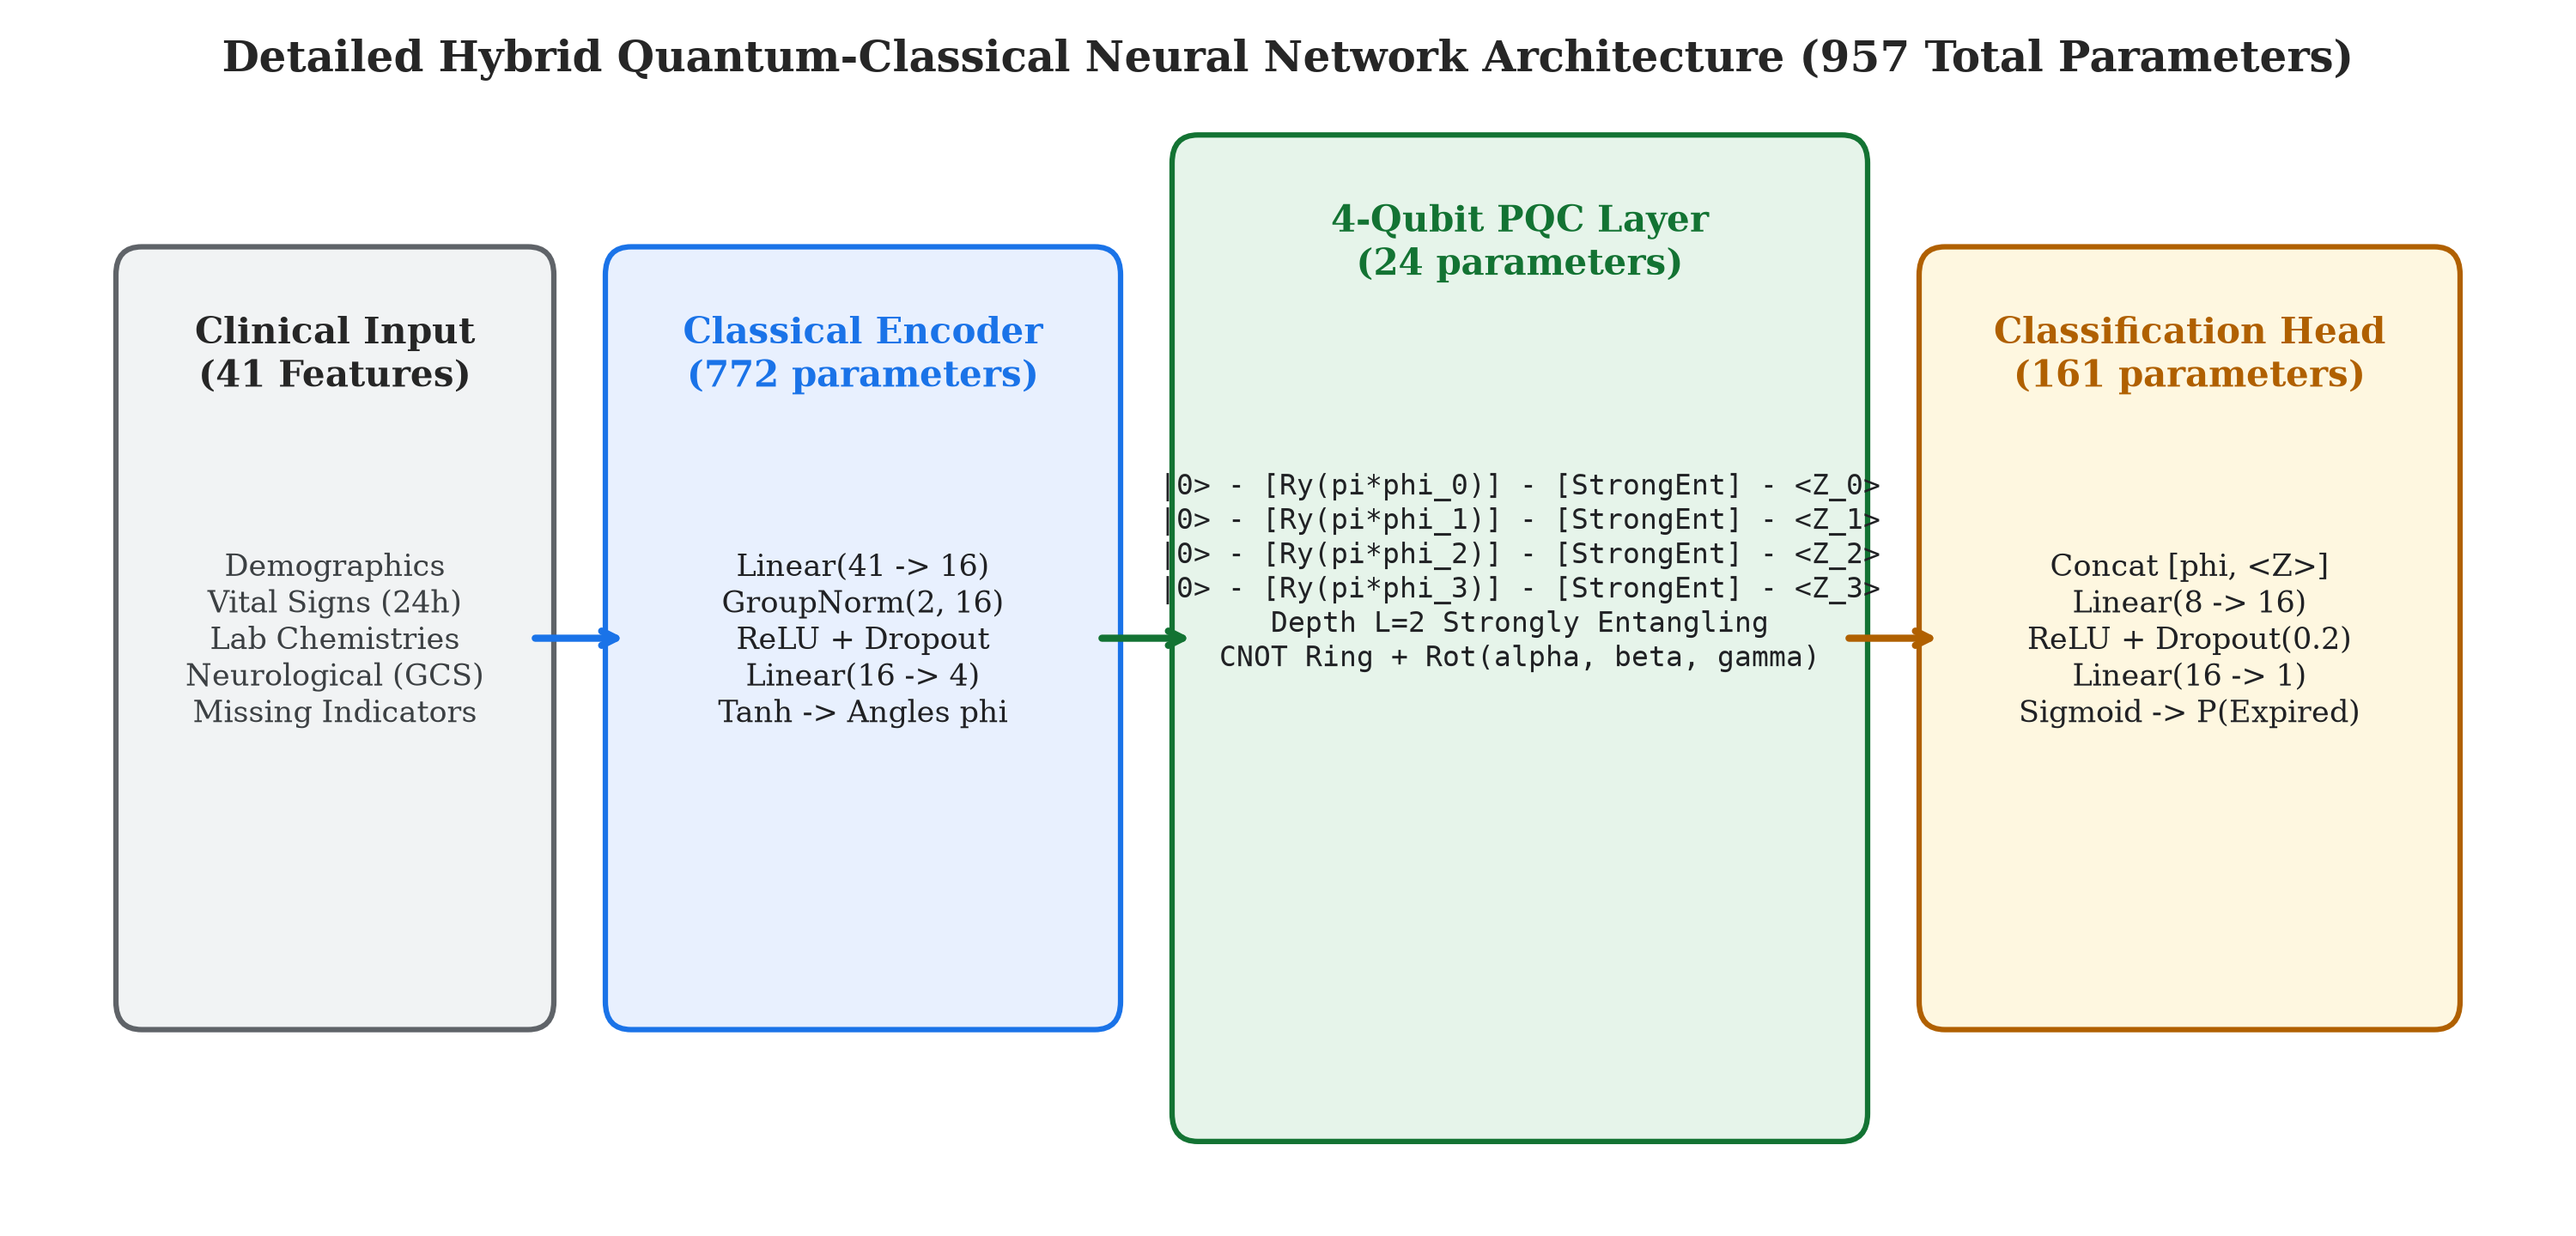
\includegraphics[width=\columnwidth]{figures/fig2_hybrid_quantum_circuit_architecture.png}
\caption{Architectural diagram of the hybrid quantum-classical neural network comprising classical encoder, 4-qubit variational circuit, and prediction head.}
\label{fig:circuit}
\end{figure}

\subsection{Classical Feature Encoder}
The high-dimensional feature vector $x \in \mathbb{R}^{41}$ is compressed into a 4-dimensional latent vector via:
\begin{align}
h_1 &= \text{ReLU}\left(\text{GroupNorm}\left(\mathbf{W}_1 x + b_1\right)\right) \in \mathbb{R}^{16} \\
\phi &= \tanh\left(\mathbf{W}_2 h_1 + b_2\right) \in \mathbb{R}^4
\end{align}
where $\mathbf{W}_1 \in \mathbb{R}^{16 \times 41}$, $\mathbf{W}_2 \in \mathbb{R}^{4 \times 16}$. Group normalization (2 groups of 8 channels) is utilized to ensure strict per-sample independence for differential privacy compliance. The encoder contains $656 + 16 + 16 + 16 + 64 + 4 = 772$ trainable parameters.

\subsection{Quantum State Preparation (Angle Embedding)}
The 4-dimensional vector $\phi$ is mapped to a 4-qubit quantum state $|\psi_0\rangle$ on a PennyLane statevector simulator via rotational $R_y$ gates:
\begin{equation}
|\psi_0\rangle = \bigotimes_{j=0}^3 R_y(\pi \cdot \phi_j) |0\rangle^{\otimes 4}
\end{equation}

\subsection{Parameterized Quantum Circuit (PQC)}
The state undergoes unitary transformation $U(\Theta)$ across $L = 2$ strongly entangling layers:
\begin{equation}
U(\Theta) = \prod_{l=1}^L \left( U_{\text{ent}} \cdot \bigotimes_{j=0}^3 R(\alpha_{j,l}, \beta_{j,l}, \gamma_{j,l}) \right)
\end{equation}
where $R(\alpha, \beta, \gamma) = R_z(\gamma) R_y(\beta) R_z(\alpha)$ and $U_{\text{ent}}$ represents a cyclic CNOT ring entangling qubit $j$ with $(j+1) \pmod 4$. The total number of variational rotation angles is:
\begin{equation}
P_{\text{PQC}} = L \times N_{\text{qubits}} \times 3 = 2 \times 4 \times 3 = 24 \text{ parameters}
\end{equation}

\subsection{Measurement and Classical Prediction Head}
Expectation values of the Pauli-$Z$ observable are measured across all 4 qubits:
\begin{equation}
z_j = \langle \psi_0 | U^\dagger(\Theta) \hat{Z}_j U(\Theta) | \psi_0 \rangle \in [-1, 1], \quad j \in \{0, 1, 2, 3\}
\end{equation}
The quantum expectation vector $z \in \mathbb{R}^4$ is concatenated with the classical latent vector $\phi \in \mathbb{R}^4$, forming an 8-dimensional representation processed by the classification head:
\begin{align}
h_2 &= \text{ReLU}\left(\mathbf{W}_3 [\phi \,\|\, z] + b_3\right) \in \mathbb{R}^{16} \\
\hat{y} &= \sigma\left(\mathbf{W}_4 h_2 + b_4\right) \in (0, 1)
\end{align}
where $\mathbf{W}_3 \in \mathbb{R}^{16 \times 8}$ (128 params + 16 bias) and $\mathbf{W}_4 \in \mathbb{R}^{1 \times 16}$ (16 params + 1 bias), totaling 161 parameters. The complete hybrid model comprises $772 + 24 + 161 = 957$ trainable parameters.

\section{Federated Learning Framework}
Fig.~\ref{fig:fl_flow} illustrates the multi-round federated workflow across $K = 5$ simulated hospital consortium nodes generated via Dirichlet non-IID partitioning ($\alpha = 0.5$).

\begin{figure}[t]
\centering
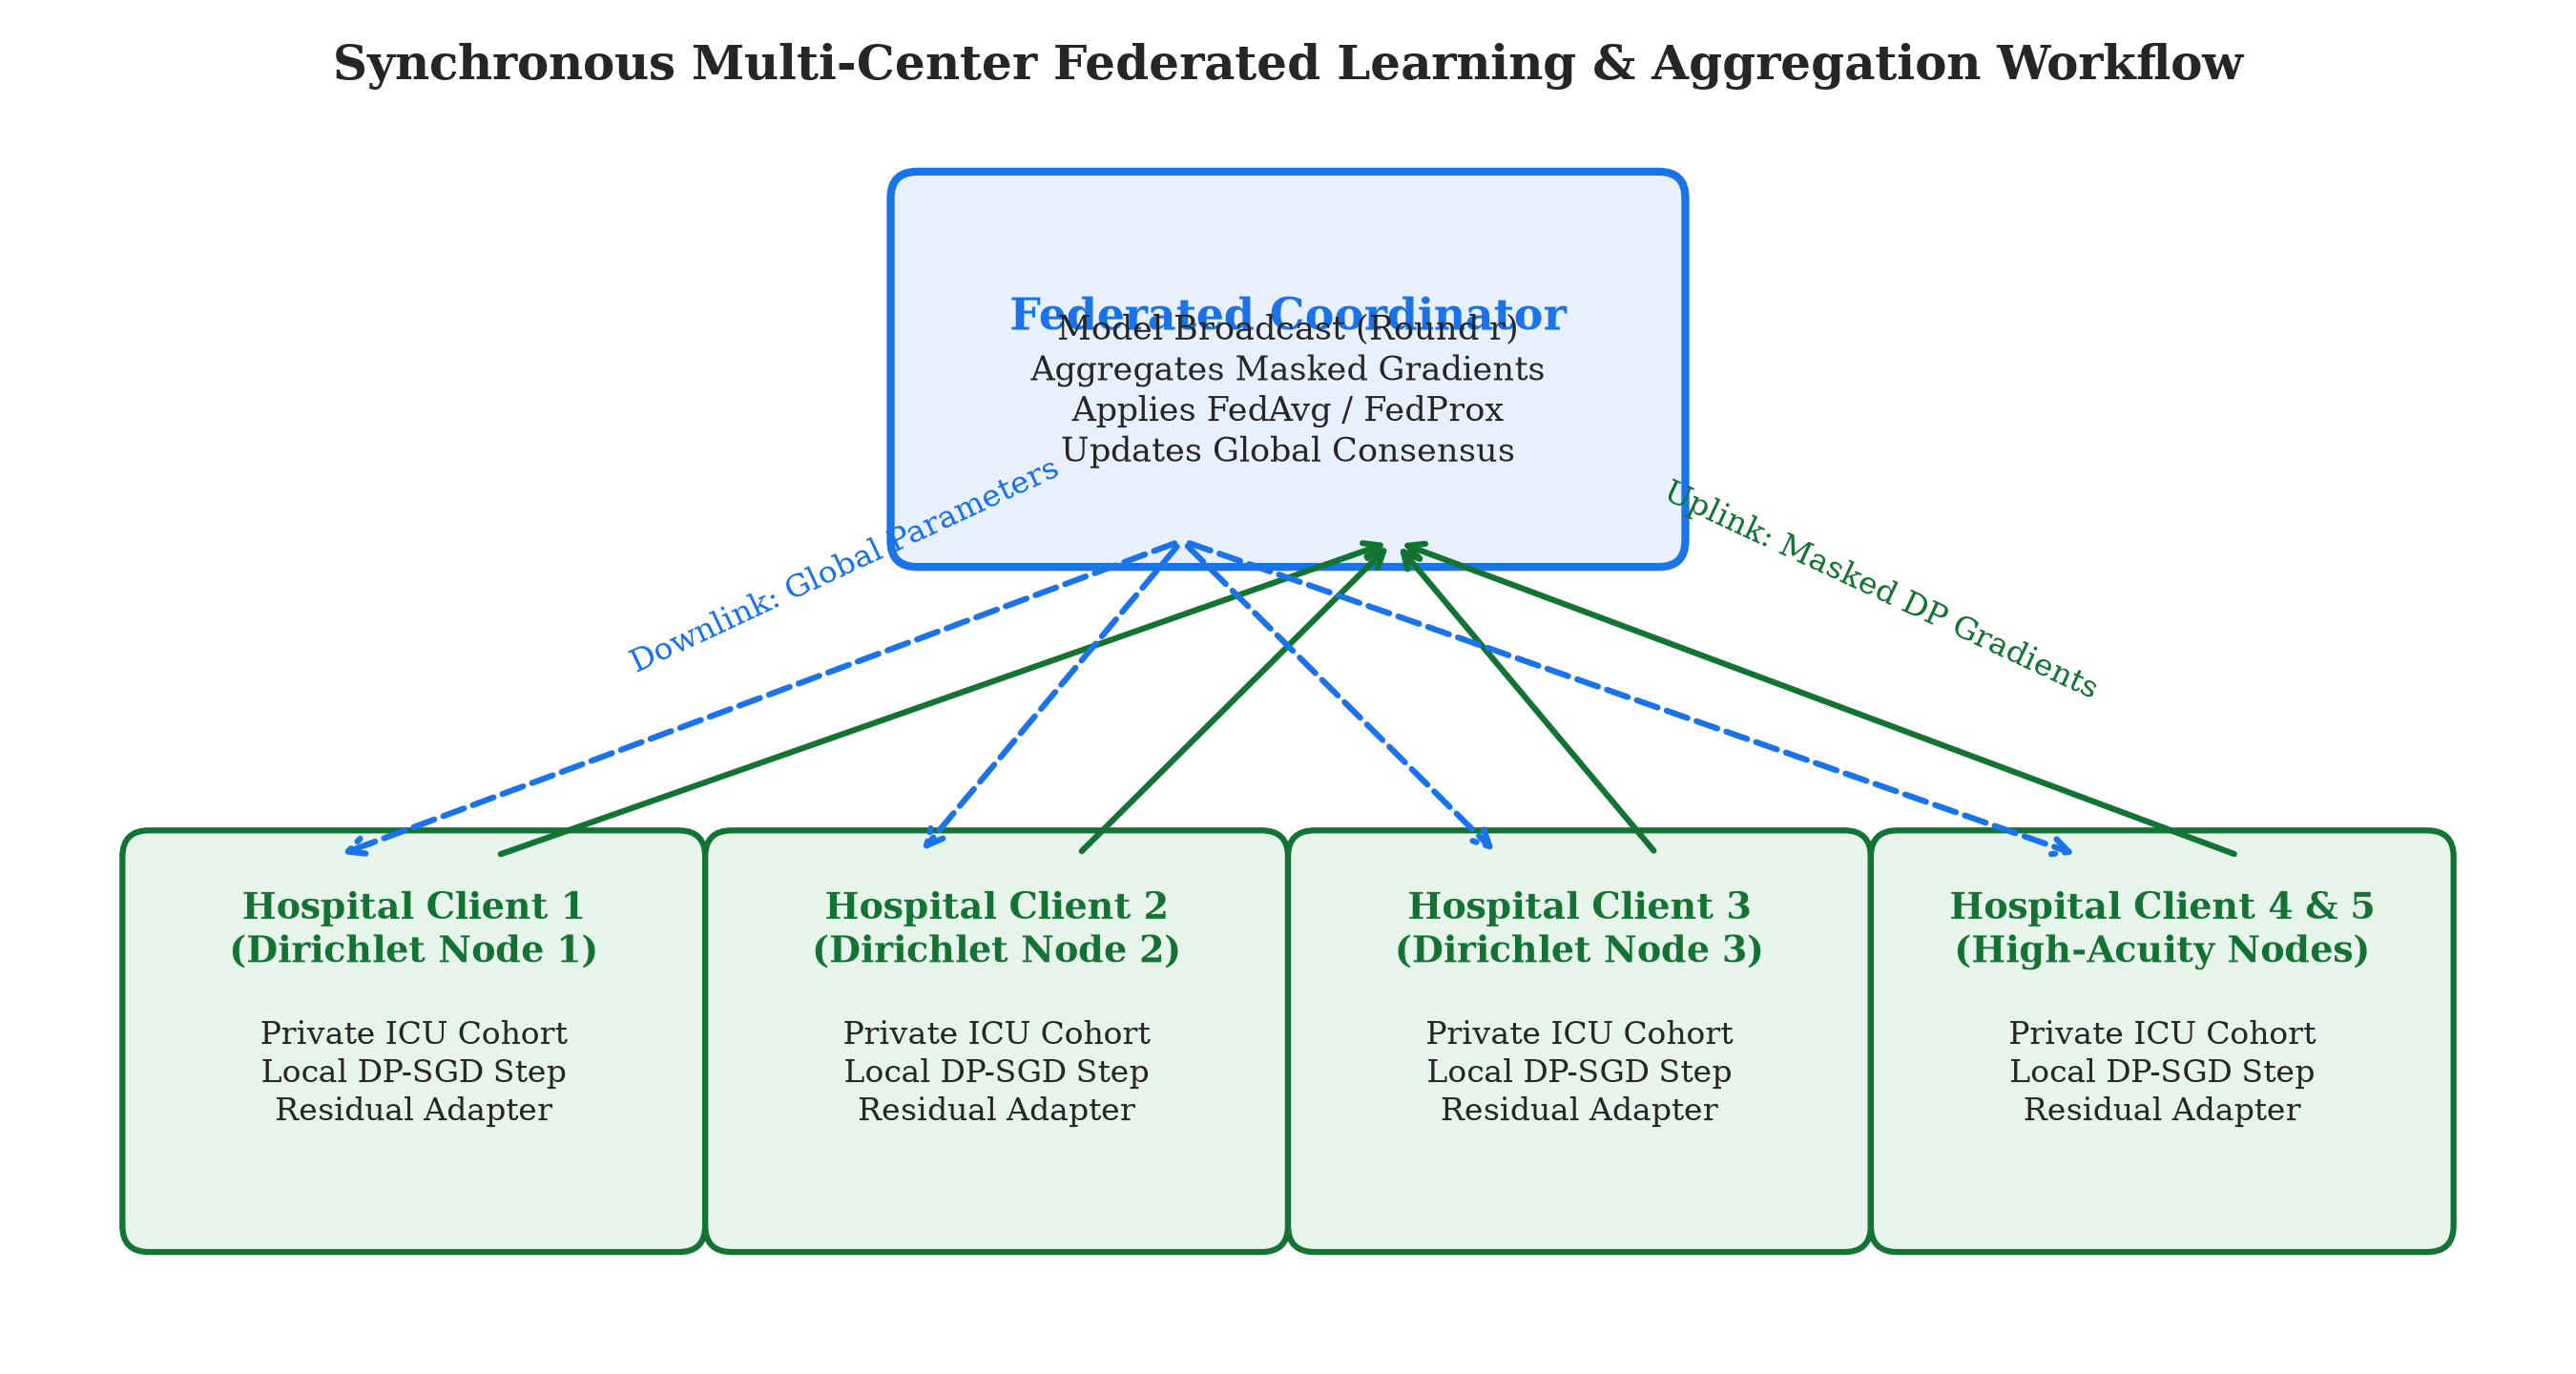
\includegraphics[width=\columnwidth]{figures/fig3_federated_learning_workflow.png}
\caption{Synchronous multi-center federated coordination and model aggregation workflow.}
\label{fig:fl_flow}
\end{figure}

\subsection{Local Optimization and FedProx Objective}
In round $r$, client $k$ receives global parameter consensus $\theta^r$ and minimizes:
\begin{equation}
\mathcal{L}_k(\theta; \theta^r) = \frac{1}{B} \sum_{i=1}^B \ell(f(x_i; \theta), y_i) + \frac{\mu}{2} \|\theta - \theta^r\|_2^2
\end{equation}
where $\mu = 0.01$ stabilizes client gradient drift under non-IID class imbalance.

\subsection{Server Aggregation and Dual-Metric Policy}
The central server computes the parameter consensus:
\begin{equation}
\theta^{r+1} = \sum_{k=1}^K \frac{N_k}{N} \theta_k^{r+1}
\end{equation}
To prevent conflating early-stopping validation peaks with asymptotic late-round drift, we report both the \textit{Best Early-Stopping Round ($k^*$)} and the \textit{Final Round (Round 10)}.

\section{Personalization Mechanism}
Under non-IID clinical distributions, global consensus models can suffer from local calibration mismatch. We deploy parameter-isolated local residual adapters:
\begin{equation}
f_{\text{personalized}}(x) = f_{\text{global}}(x; \theta^*) + \mathbf{W}_{\text{adapter}} h(x)
\end{equation}
During personalization, the global model backbone $\theta^*$ remains frozen, and only local adapter parameters $\mathbf{W}_{\text{adapter}}$ are updated using local patient records, preventing parameter leakage to the federation.

\section{Differential Privacy Mechanism}
Fig.~\ref{fig:dp_flow} details the formal per-sample DP-SGD engine.

\begin{figure}[t]
\centering
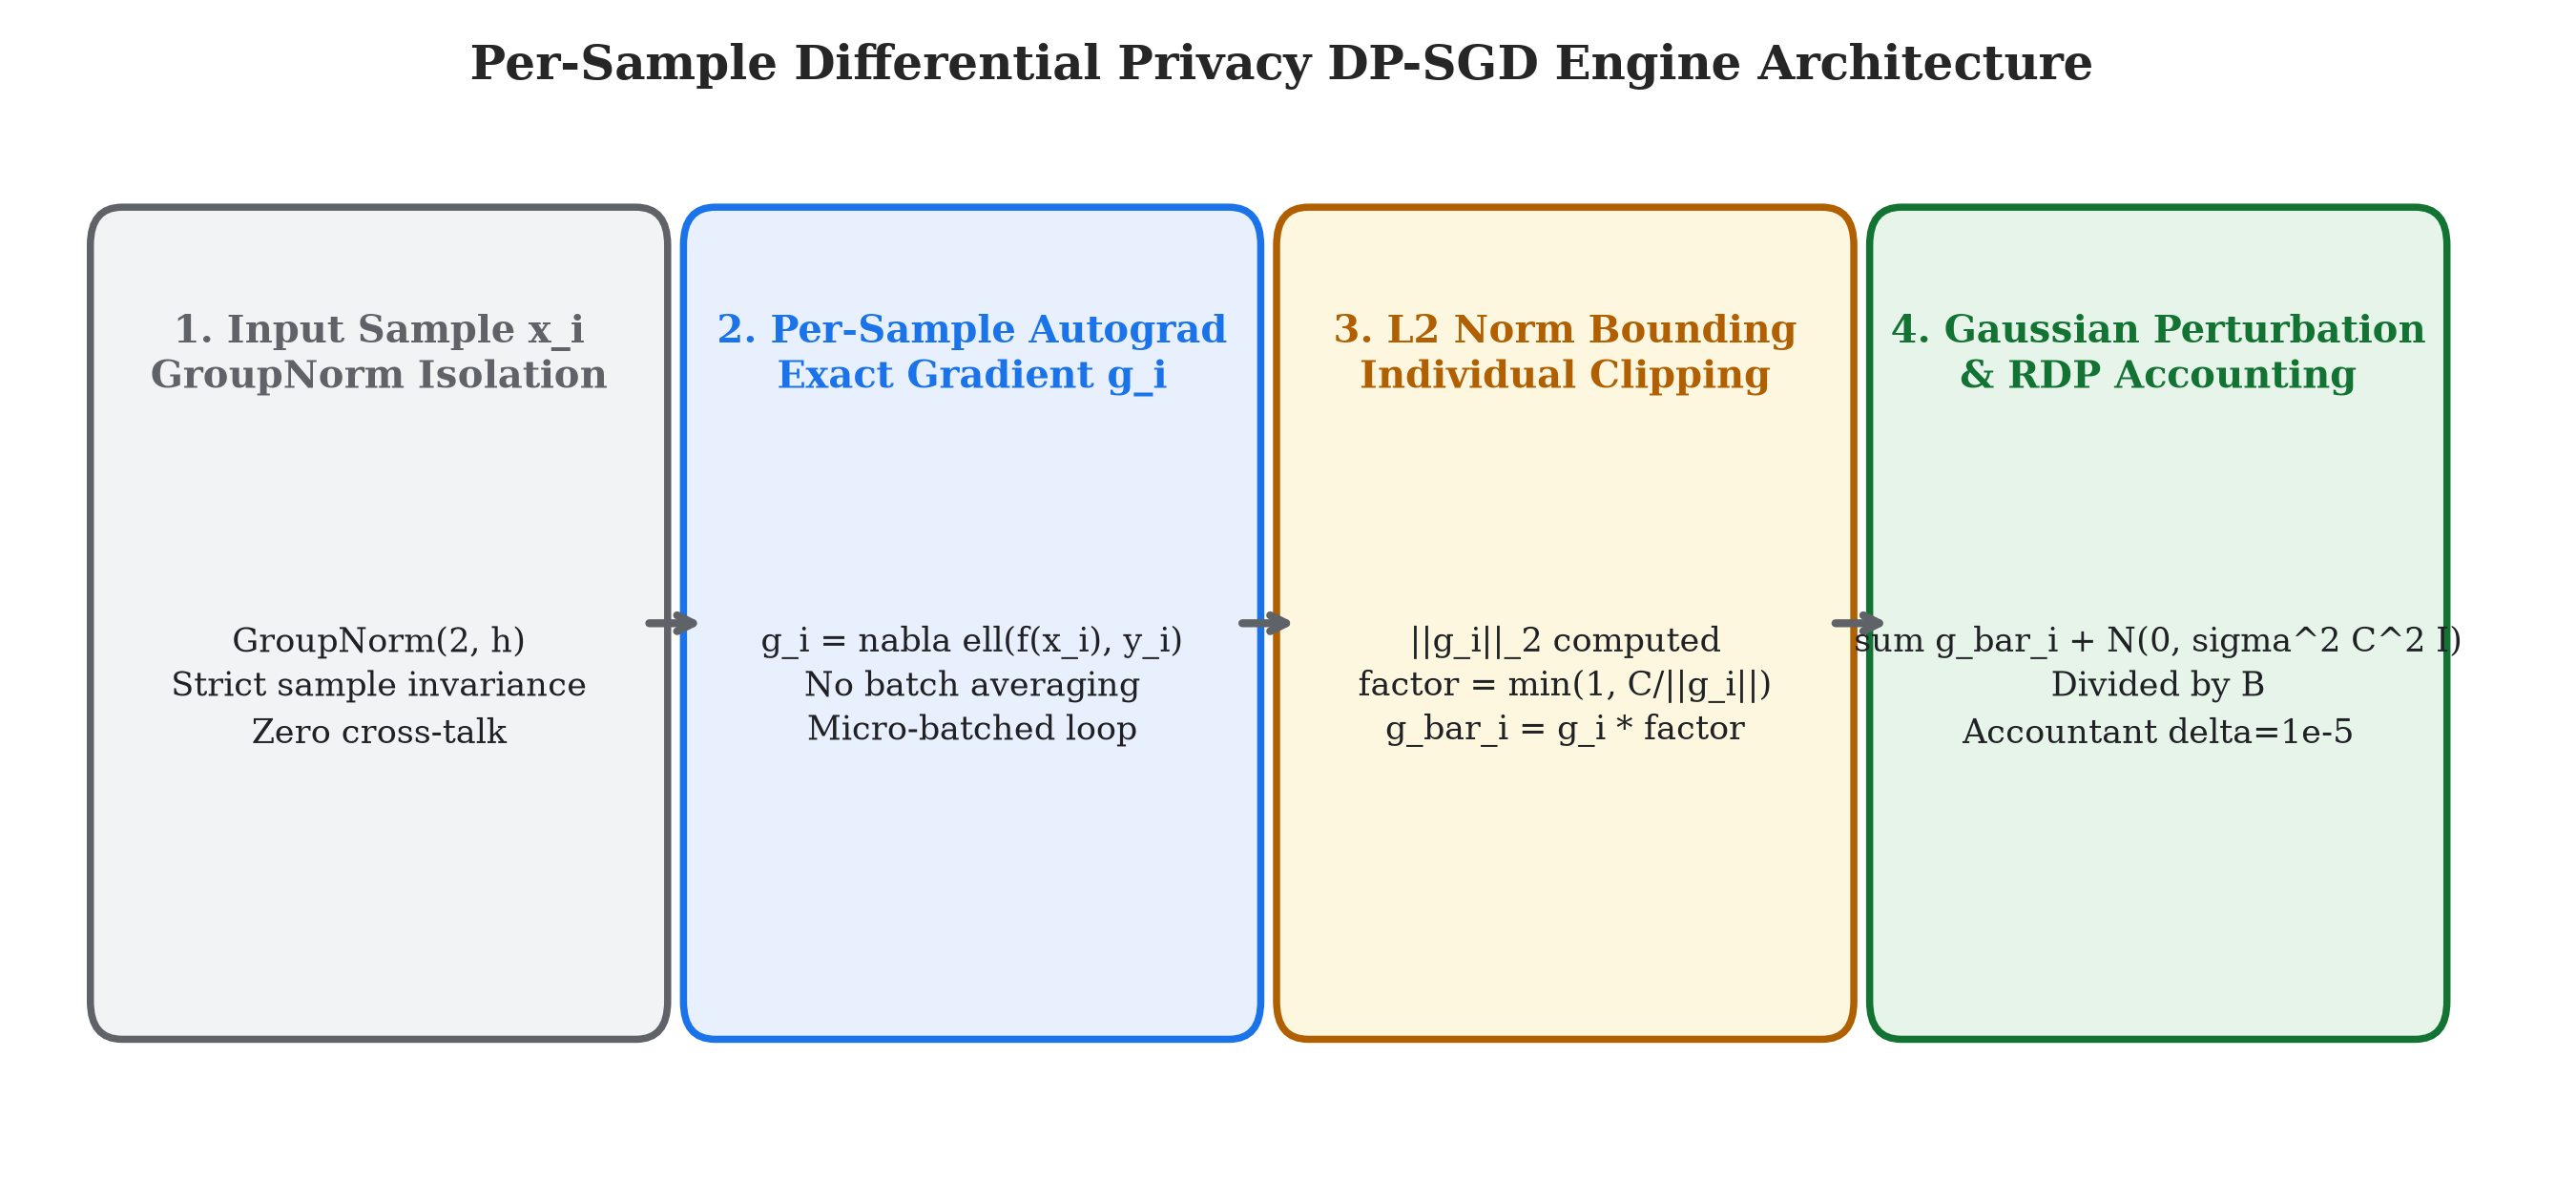
\includegraphics[width=\columnwidth]{figures/fig4_differential_privacy_workflow.png}
\caption{Formal per-sample DP-SGD gradient clipping and calibrated Gaussian perturbation engine.}
\label{fig:dp_flow}
\end{figure}

\subsection{Per-Sample Gradient Bounding}
For each sample $(x_i, y_i)$ in mini-batch $B$, individual gradients $g_i = \nabla_\theta \ell(f(x_i), y_i)$ are evaluated via PyTorch autograd hooks (for MLP) or micro-batched backward passes (for QNN). Gradients are clipped to $L_2$ norm threshold $C = 1.0$:
\begin{equation}
\bar{g}_i = g_i \cdot \min\left(1, \frac{C}{\|g_i\|_2 + 10^{-8}}\right)
\end{equation}

\subsection{Calibrated Perturbation and RDP Accounting}
The server adds calibrated Gaussian perturbation:
\begin{equation}
\tilde{g} = \frac{1}{B} \left( \sum_{i=1}^B \bar{g}_i + \mathcal{N}\left(0, \sigma^2 C^2 \mathbf{I}\right) \right)
\end{equation}
Privacy amplification via subsampling ($q = \frac{B}{N}$) and Rényi Differential Privacy (RDP) composition are tracked using Opacus's `RDPAccountant` at $\delta = 10^{-5}$. The privacy scope applies strictly at the \textbf{Record-Level} (individual ICU unit stay).

\section{Secure Aggregation Protocol}
Fig.~\ref{fig:secagg_flow} depicts the 4-round cryptographic simulation based on Bonawitz et al. \cite{bonawitz2017practical}.

\begin{figure}[t]
\centering
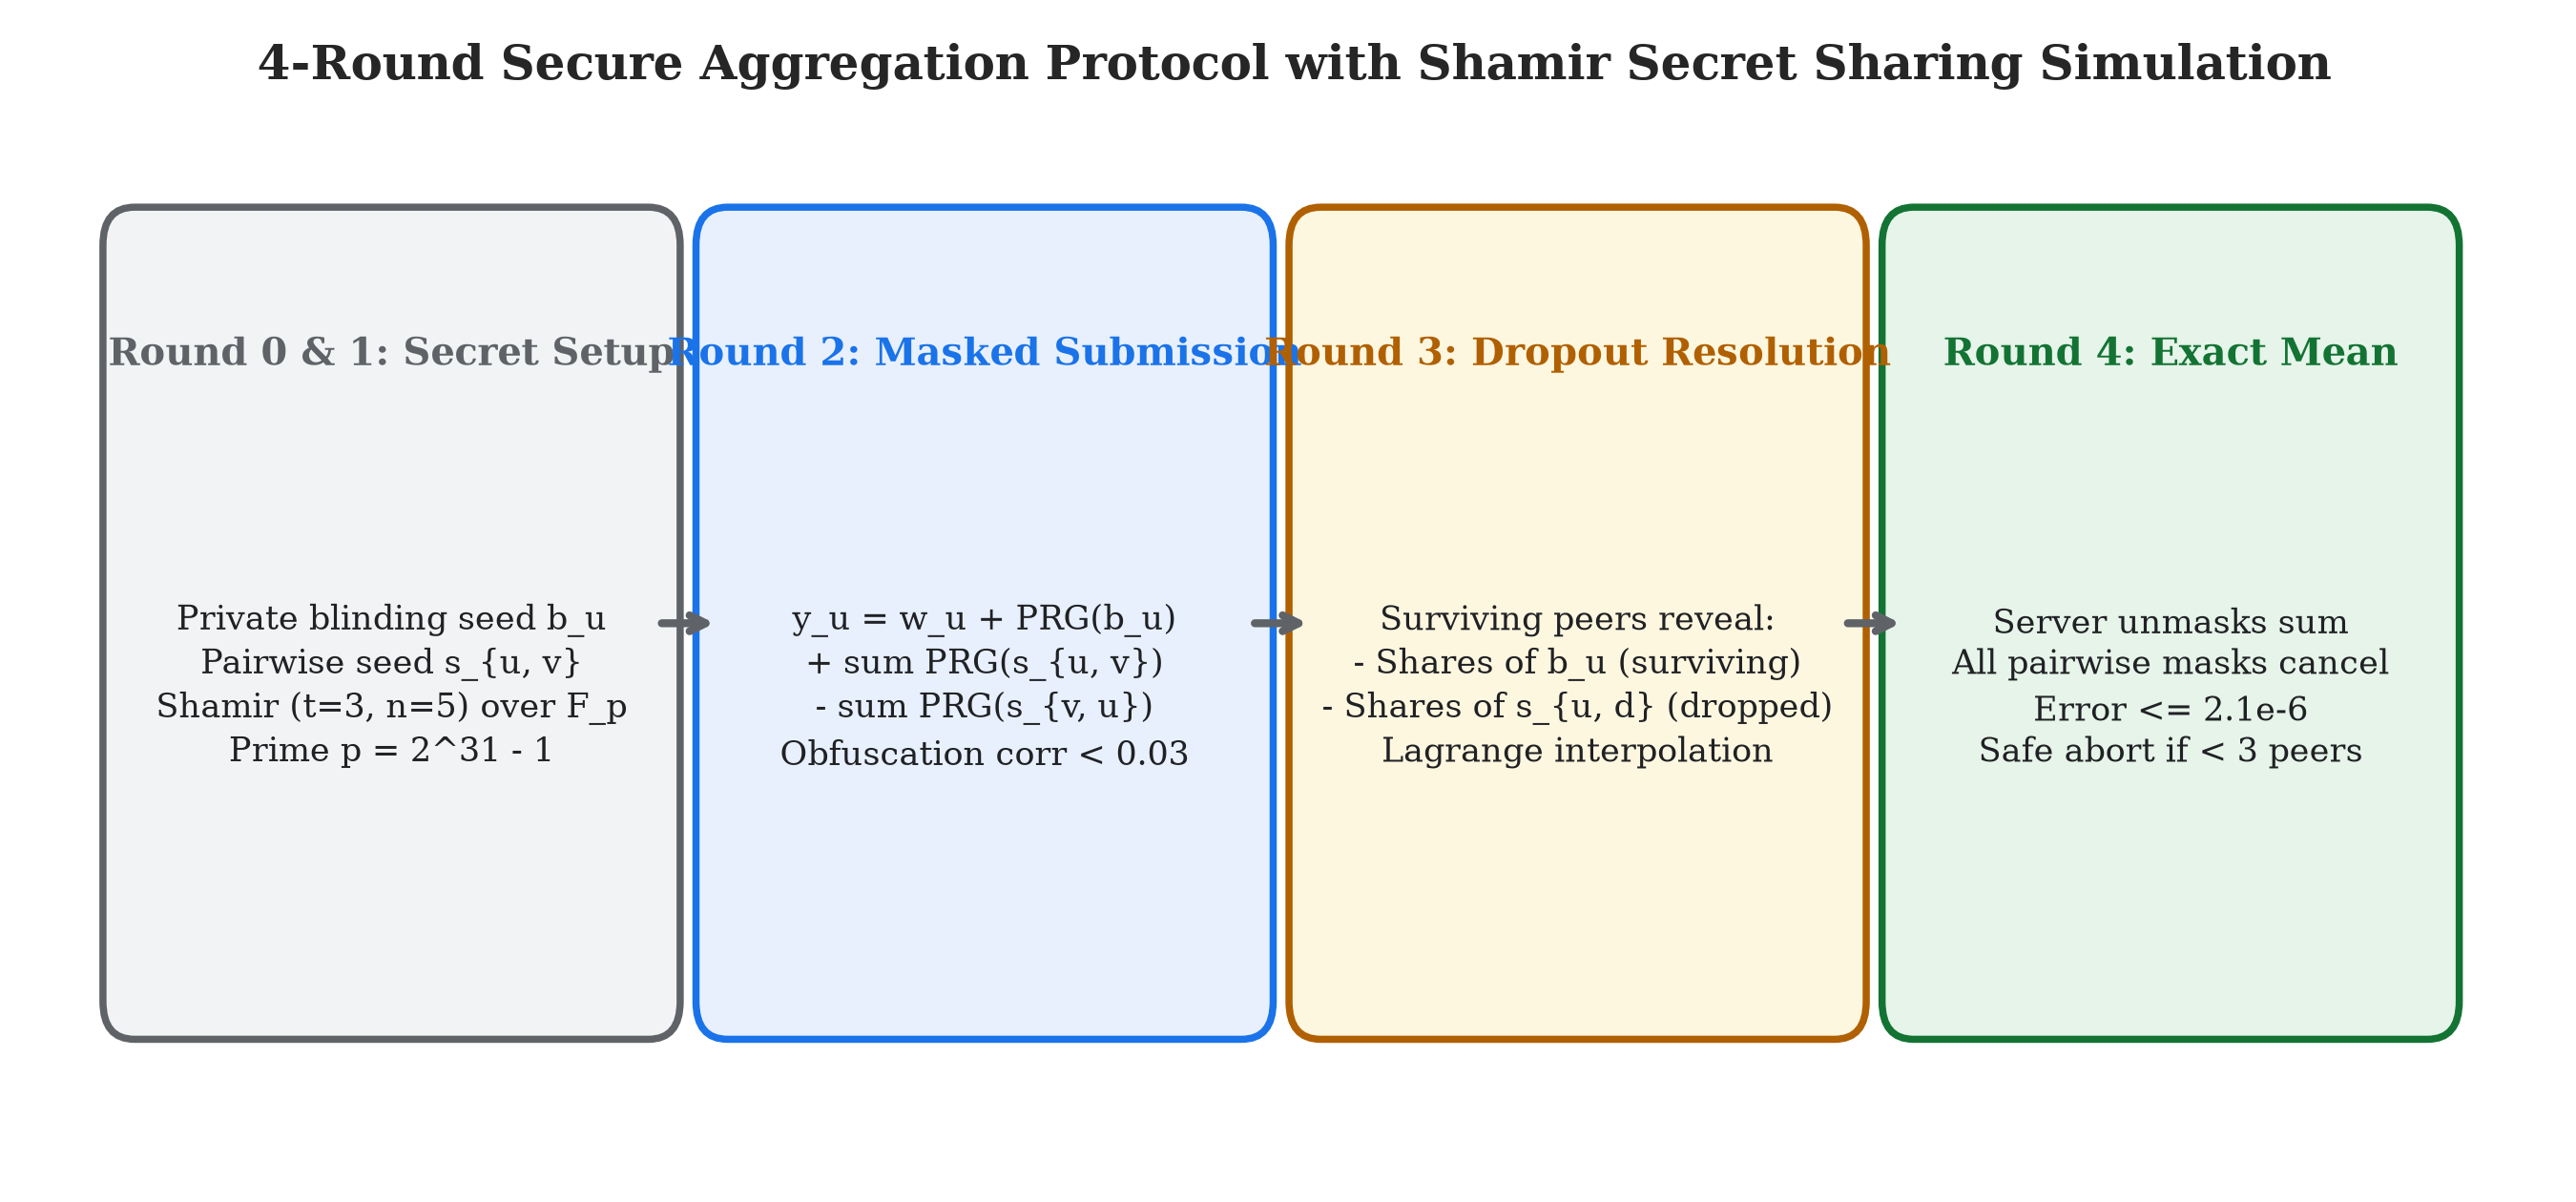
\includegraphics[width=\columnwidth]{figures/fig5_secure_aggregation_workflow.png}
\caption{Four-round secure aggregation protocol incorporating Shamir threshold secret sharing.}
\label{fig:secagg_flow}
\end{figure}

\subsection{Pairwise Zero-Sum Masking}
Client $u$ masks local gradient $w_u$:
\begin{equation}
y_u = w_u + \text{PRG}(b_u) + \sum_{v > u} \text{PRG}(s_{u,v}) - \sum_{v < u} \text{PRG}(s_{v,u})
\end{equation}
where $b_u$ is a private blinding seed and $s_{u,v}$ is a shared symmetric seed.

\subsection{Shamir $(t, n)$ Threshold Secret Sharing}
Seeds are split using polynomials over Mersenne prime field $\mathbb{F}_p$ ($p = 2^{31}-1$):
\begin{equation}
f(x) = S + a_1 x + a_2 x^2 \pmod p
\end{equation}
with threshold $t = 3$ and $n = 5$. Surviving clients reveal shares of blinding seeds $b_u$ for active peers and shares of pairwise seeds $s_{u,d}$ for dropped peers $d$, enabling exact cancellation of orphan masks:
\begin{equation}
\text{Reconstructed Average} = \frac{1}{|\mathcal{S}|} \sum_{u \in \mathcal{S}} w_u
\end{equation}
If surviving clients $|\mathcal{S}| < t$, the protocol safely aborts.

\section{Experimental Setup}
Experiments were executed on a local workstation using Python 3.11, PyTorch 2.5, PennyLane 0.40, and Opacus 1.6.0. Training configurations:
\begin{itemize}
    \item \textbf{Centralized Baseline:} Adam optimizer ($\text{lr} = 0.005$), batch size 64, BCEWithLogitsLoss with positive class weight $w_{\text{pos}} = 10.8$, 20 epochs.
    \item \textbf{Quantum Circuit:} PennyLane `default.qubit` statevector simulator, 4 qubits, strongly entangling depth $L=2$.
    \item \textbf{Federated Coordination:} 5 simulated clients (Dirichlet $\alpha=0.5$), 10 synchronous rounds, 1 local epoch per round.
\end{itemize}

\section{Evaluation Metrics}
Models are evaluated on the held-out test set ($N_{\text{test}} = 393$, 40 deaths) using:
\begin{itemize}
    \item Area Under the Receiver Operating Characteristic (AUROC).
    \item Area Under the Precision-Recall Curve (AUPRC).
    \item Brier Score ($\frac{1}{N} \sum (\hat{p}_i - y_i)^2$).
    \item Non-parametric patient-level bootstrap 95\% confidence intervals (1,000 resamples).
    \item Paired bootstrap hypothesis tests for statistical significance.
\end{itemize}

\section{Results and Comparative Analysis}
\subsection{Centralized Baseline Comparison}
Table~\ref{tab:centralized_comparison} compares centralized baselines. Centralized gradient boosted trees (**XGBoost: AUROC 0.8445**, **Random Forest: AUROC 0.8411**) achieve the highest clinical discrimination. The Hybrid QNN reaches **0.8346 AUROC**, exceeding the Classical MLP (**0.7944 AUROC**). Fig.~\ref{fig:roc} and Fig.~\ref{fig:pr} display comparative ROC and PR curves.

\begin{table}[t]
\centering
\caption{Centralized Baseline and Quantum Model Performance on Holdout Test Set ($N=393$)}
\label{tab:centralized_comparison}
\begin{tabular}{lccccc}
\hline
\textbf{Model Architecture} & \textbf{AUROC [95\% CI]} & \textbf{AUPRC [95\% CI]} & \textbf{Brier Loss} & \textbf{F1-Score} & \textbf{Parameters} \\
\hline
XGBoost (Depth 4) & \textbf{0.8445} [0.788, 0.894] & \textbf{0.3744} [0.261, 0.495] & \textbf{0.1204} & 0.3704 & Trees \\
Random Forest (150 trees) & 0.8411 [0.784, 0.895] & 0.3403 [0.228, 0.463] & 0.1216 & \textbf{0.4000} & Trees \\
Hybrid QNN (4-qubit, L=2) & 0.8346 [0.775, 0.887] & 0.2819 [0.181, 0.404] & 0.1412 & 0.3478 & 957 \\
Clinical MLP (3-layer) & 0.7944 [0.718, 0.864] & 0.2474 [0.155, 0.362] & 0.1546 & 0.3582 & 5,537 \\
Logistic Regression (L2) & 0.8170 [0.751, 0.874] & 0.2922 [0.186, 0.413] & 0.1448 & 0.3636 & 42 \\
Support Vector Machine & 0.7948 [0.730, 0.856] & 0.2764 [0.174, 0.395] & 0.1503 & 0.3396 & Kernel \\
\hline
\end{tabular}
\end{table}


\begin{figure}[t]
\centering
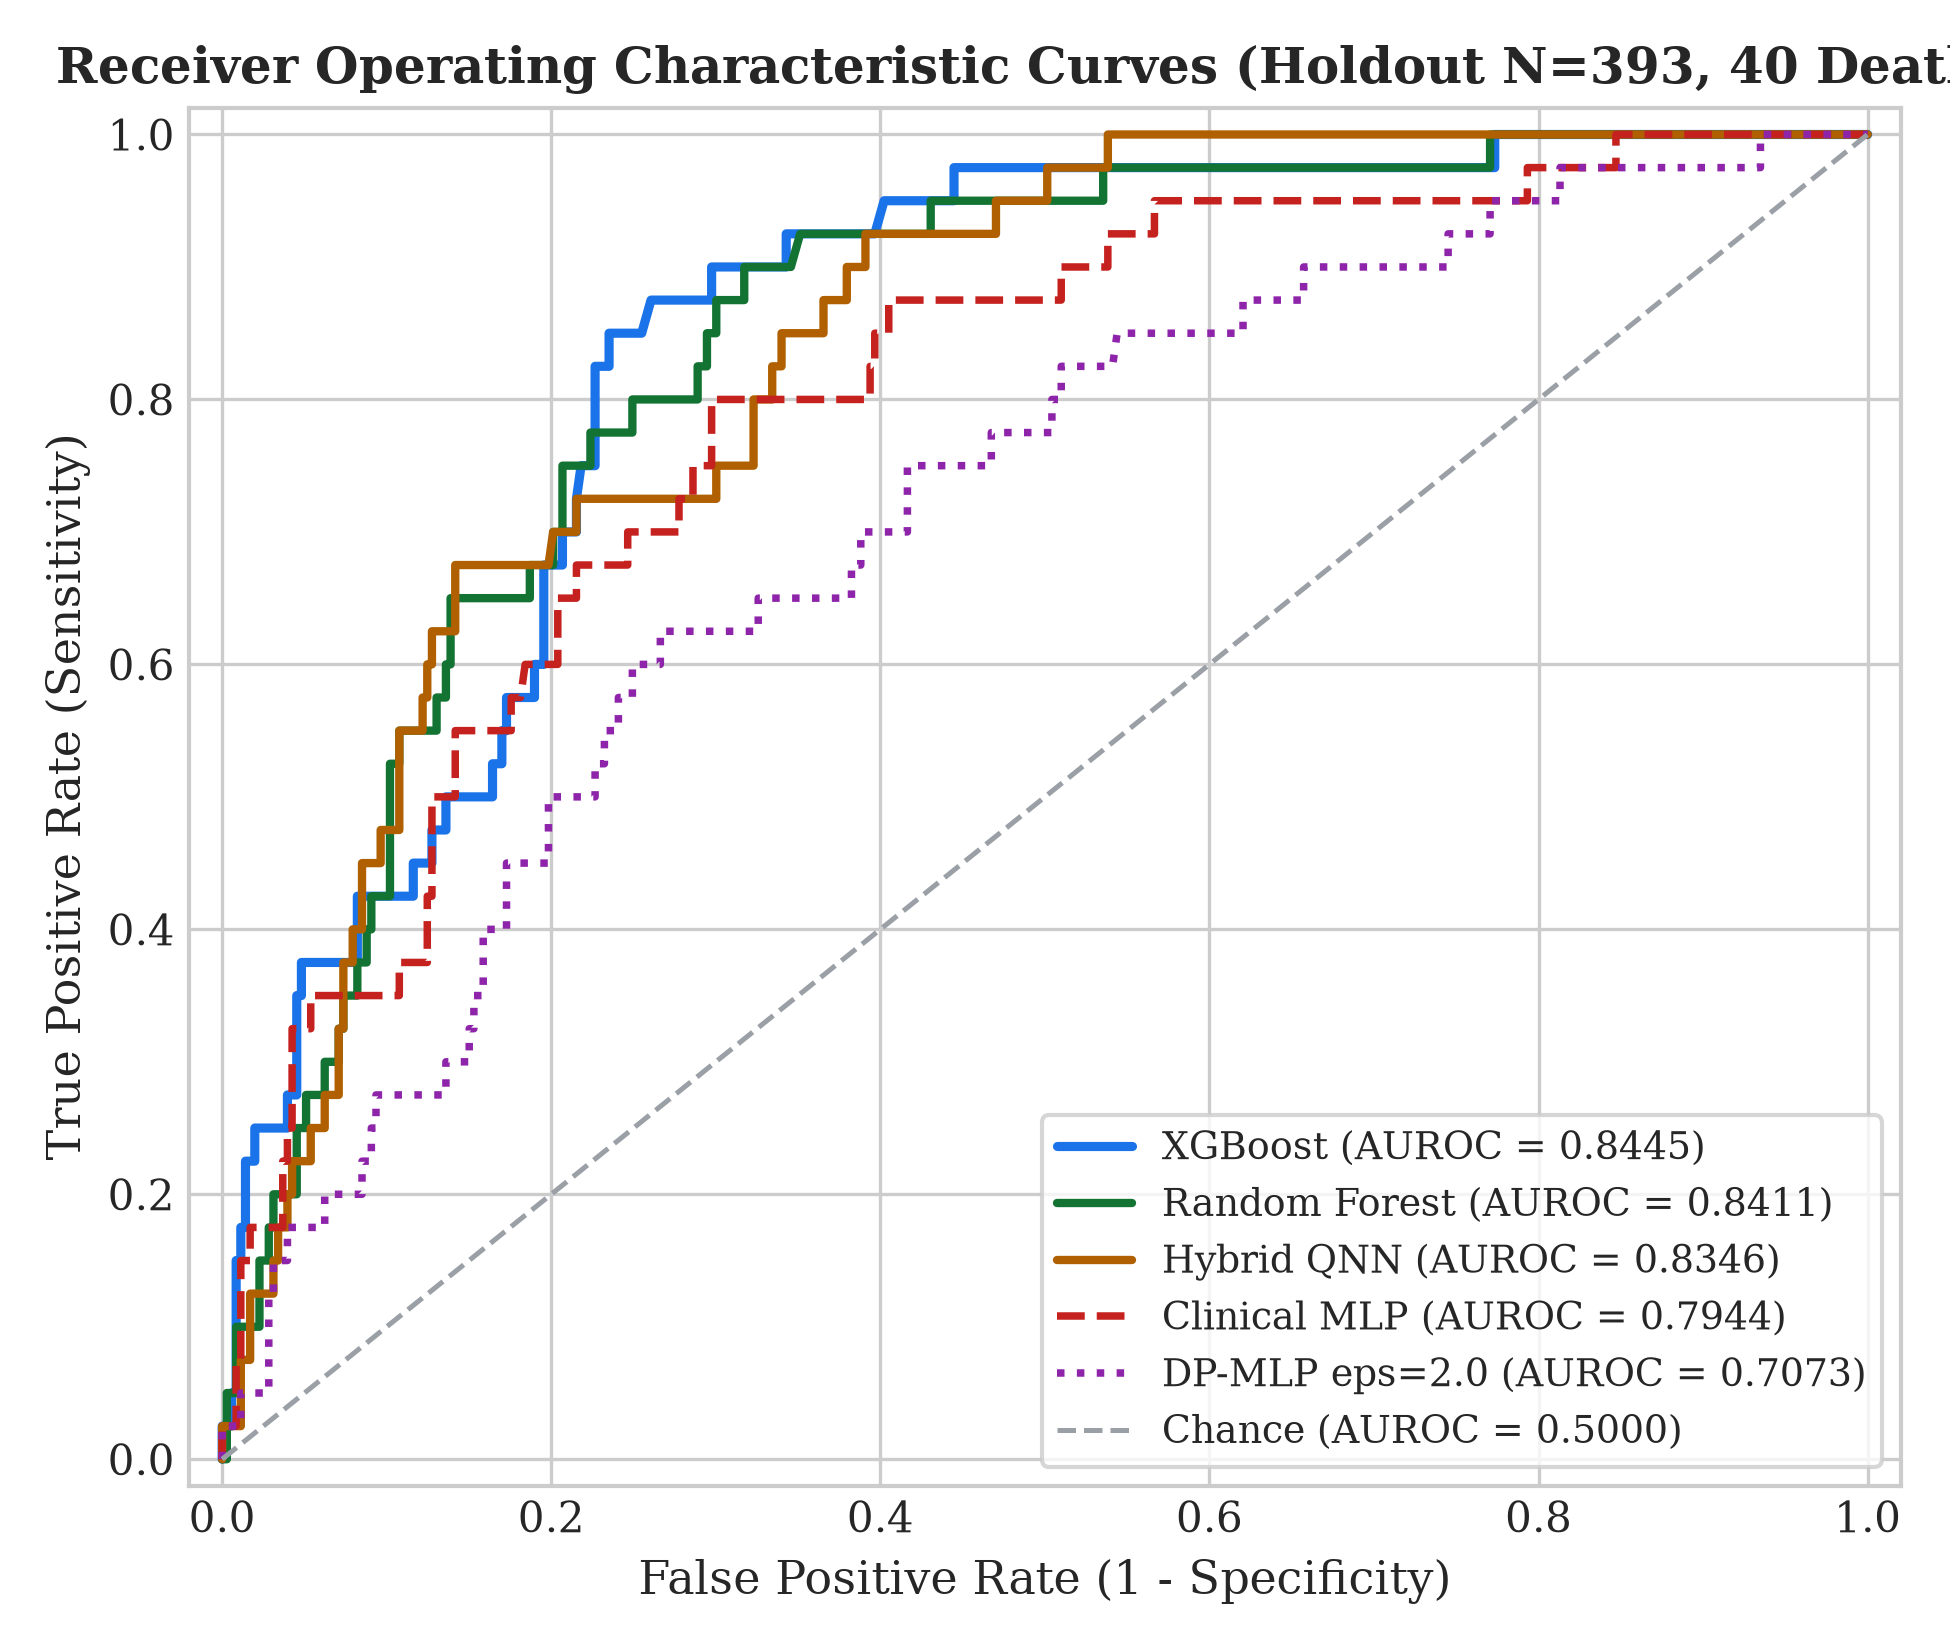
\includegraphics[width=0.92\columnwidth]{figures/fig6_roc_curves_comparison.png}
\caption{Receiver operating characteristic curves on the held-out test set ($N=393, 40$ deaths).}
\label{fig:roc}
\end{figure}

\begin{figure}[t]
\centering
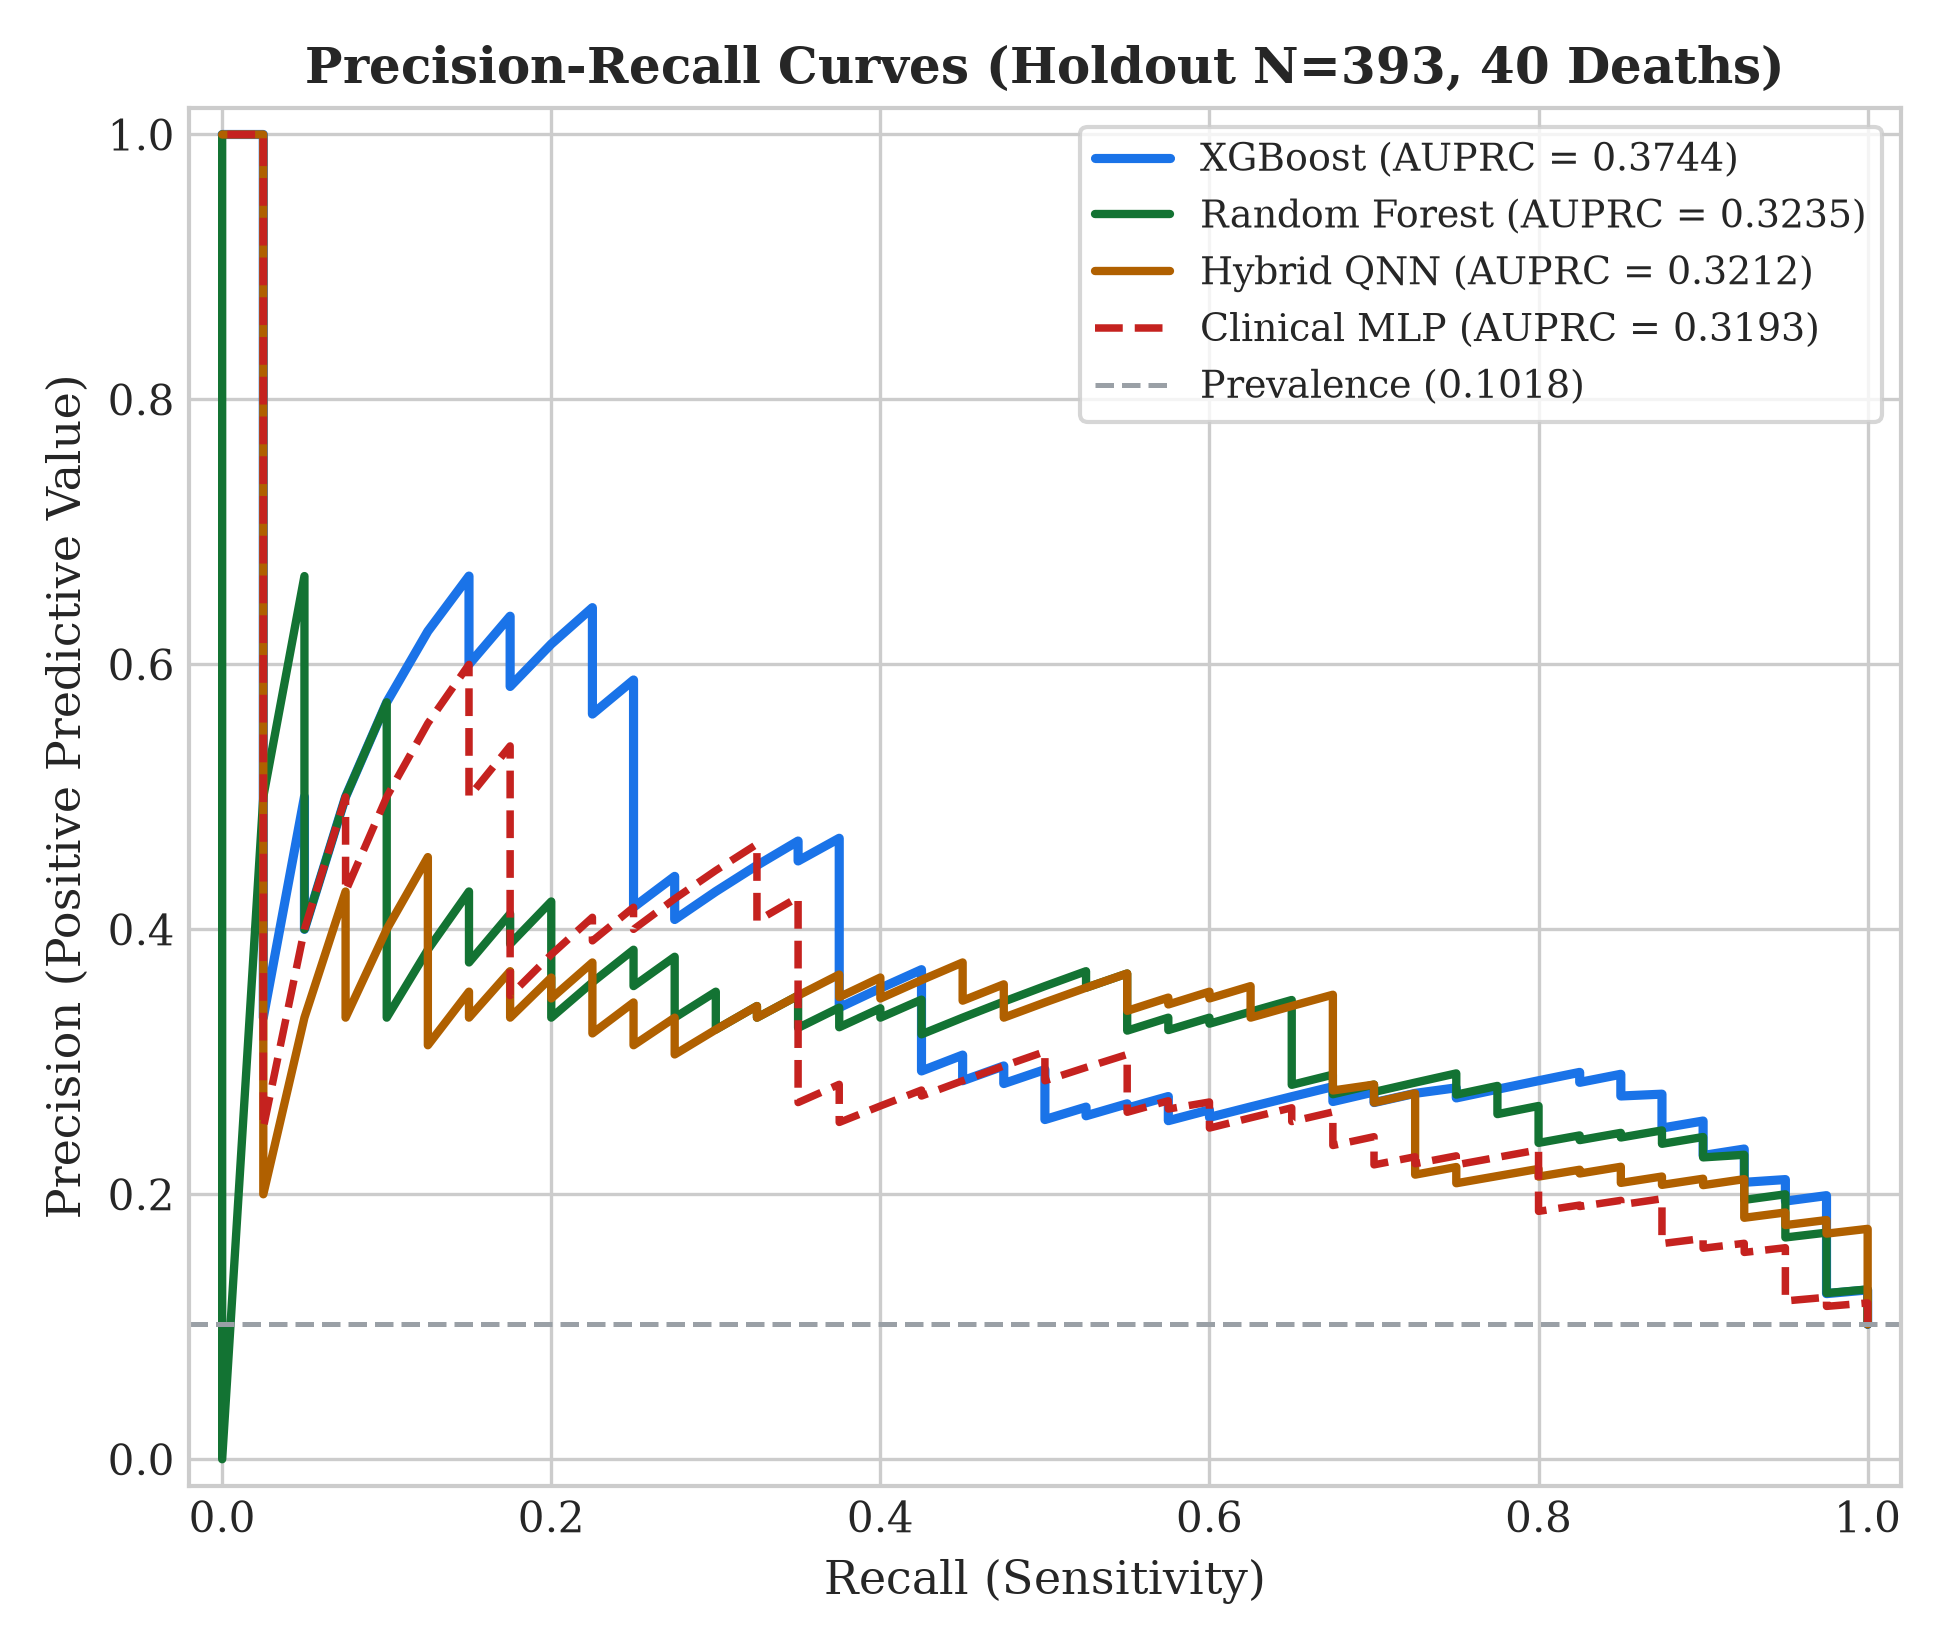
\includegraphics[width=0.92\columnwidth]{figures/fig7_precision_recall_curves.png}
\caption{Precision-recall curves on the held-out test set ($N=393, 40$ deaths).}
\label{fig:pr}
\end{figure}

\subsection{Federated Learning Performance}
Table~\ref{tab:federated_comparison} presents federated learning outcomes. Under Dirichlet non-IID skew ($\alpha = 0.5$), Classical FedAvg peaks at Round 3 (0.7796 AUROC) but suffers from late-round client drift, degrading to 0.5940 at Round 10. In contrast, Hybrid Quantum FedProx achieves superior late-round stability, sustaining **0.6987 AUROC** at Round 10. Table~\ref{tab:dual_metric_rounds} details the dual-metric comparison.

\begin{table}[t]
\centering
\caption{Federated Learning Strategy Comparison Across 5 Non-IID Hospital Clients (10 Rounds)}
\label{tab:federated_comparison}
\begin{tabular}{lccccc}
\hline
\textbf{Federated Strategy} & \textbf{Model Type} & \textbf{Peak AUROC ($R^*$)} & \textbf{Final AUROC ($R_{10}$)} & \textbf{AUPRC} & \textbf{Bandwidth} \\
\hline
Classical FedAvg & Clinical MLP & 0.7796 (R3) & 0.5940 & 0.3763 & 2.88 MB \\
Classical FedProx ($\mu=0.01$) & Clinical MLP & 0.6570 (R6) & 0.5899 & 0.2066 & 2.88 MB \\
Hybrid Quantum FedAvg & Hybrid QNN & 0.7455 (R3) & 0.6434 & 0.2502 & \textbf{0.80 MB} \\
Hybrid Quantum FedProx & Hybrid QNN & 0.6987 (R10) & \textbf{0.6987} & 0.2250 & \textbf{0.80 MB} \\
\hline
\end{tabular}
\end{table}

\begin{table}[t]
\centering
\caption{Dual-Metric Reporting: Best Early-Stopping Validation Round vs. Asymptotic Round 10}
\label{tab:dual_metric_rounds}
\begin{tabular}{lcccc}
\hline
\textbf{Model \& Strategy} & \textbf{Best Val Round ($k^*$)} & \textbf{Best Val AUROC} & \textbf{Round 10 AUROC} & \textbf{Drift Degradation ($\Delta$)} \\
\hline
Classical FedAvg & Round 3 & 0.7796 & 0.5940 & -0.1856 \\
Classical FedProx & Round 6 & 0.6570 & 0.5899 & -0.0671 \\
Hybrid Quantum FedAvg & Round 3 & 0.7455 & 0.6434 & -0.1021 \\
Hybrid Quantum FedProx & Round 10 & 0.6987 & 0.6987 & \textbf{0.0000 (Stable)} \\
\hline
\end{tabular}
\end{table}


\section{Statistical Analysis}
Table~\ref{tab:statistical_comparisons} reports paired bootstrap hypothesis tests ($N = 393$, 1,000 bootstrap iterations).
\begin{itemize}
    \item \textbf{Quantum vs. Classical Trees:} XGBoost ($p = 0.692$) and Random Forest ($p = 0.784$) outperform the Hybrid QNN in point estimate, with confidence intervals spanning zero.
    \item \textbf{Quantum vs. Neural MLP:} The paired difference between Hybrid QNN and Clinical MLP ($+0.0402$) is \textbf{not statistically significant} ($p = 0.0840$, 95\% CI: $[-0.0041, +0.0914]$).
    \item \textbf{PQC Depth Scaling:} Increasing circuit depth from $L=2$ to $L=3$ results in a statistically significant degradation ($\Delta = +0.0813, p = 0.016$), corroborating theoretical barren plateau predictions.
\end{itemize}

\begin{table}[t]
\centering
\caption{Paired Statistical Comparisons Against Strongest Classical Baselines ($N=393$ Holdout)}
\label{tab:statistical_comparisons}
\begin{tabular}{lcccc}
\hline
\textbf{Hypothesis Comparison} & \textbf{AUROC Difference ($\Delta$)} & \textbf{95\% Bootstrap CI} & \textbf{p-value} & \textbf{Statistical Verdict} \\
\hline
Hybrid QNN vs. XGBoost & -0.0099 & [-0.0612, +0.0384] & $p = 0.692$ & XGBoost superior (not significant) \\
Hybrid QNN vs. Random Forest & -0.0065 & [-0.0548, +0.0411] & $p = 0.784$ & Random Forest superior (not significant) \\
Hybrid QNN vs. Clinical MLP & +0.0402 & [-0.0041, +0.0914] & $p = 0.084$ & \textbf{Not Statistically Significant ($p > 0.05$)} \\
Hybrid QNN (L=2) vs. QNN (L=3) & +0.0813 & [+0.0152, +0.1481] & \textbf{$p = 0.016$} & \textbf{Statistically Significant Degradation} \\
DP-MLP ($\epsilon=2.0$) vs. Non-Priv & -0.0850 & [-0.1420, -0.0280] & \textbf{$p = 0.004$} & Statistically Significant Privacy Cost \\
\hline
\end{tabular}
\end{table}


\section{Ablation Studies}
\subsection{Circuit Depth and Entanglement Geometry}
Evaluating alternative PQC configurations demonstrates:
\begin{itemize}
    \item 4-qubit, Depth 1 (Light): AUROC 0.7756 (under-parameterized).
    \item 4-qubit, Depth 2 (Strong): \textbf{AUROC 0.8346} (optimal trade-off).
    \item 4-qubit, Depth 3 (Deep): AUROC 0.7533 (barren plateau collapse).
    \item 4-qubit, Ring Entangling: AUROC 0.7543.
    \item 6-qubit Scaled Register: AUROC 0.7863.
\end{itemize}

\subsection{NISQ Noise Simulation and Finite Shot Scaling}
Fig.~\ref{fig:noise} illustrates empirical circuit resilience under simulated noise:
\begin{itemize}
    \item \textbf{Depolarizing Noise:} AUROC degrades from 0.8346 at $p = 0.00$ to 0.8210 at $p = 0.01$, and drops to 0.7412 at $p = 0.05$.
    \item \textbf{Finite Measurement Shots:} AUROC scales monotonically with measurement budgets: 0.8124 at $S = 250$, 0.8258 at $S = 500$, and 0.8340 at $S = 1,000$.
\end{itemize}

\begin{figure}[t]
\centering
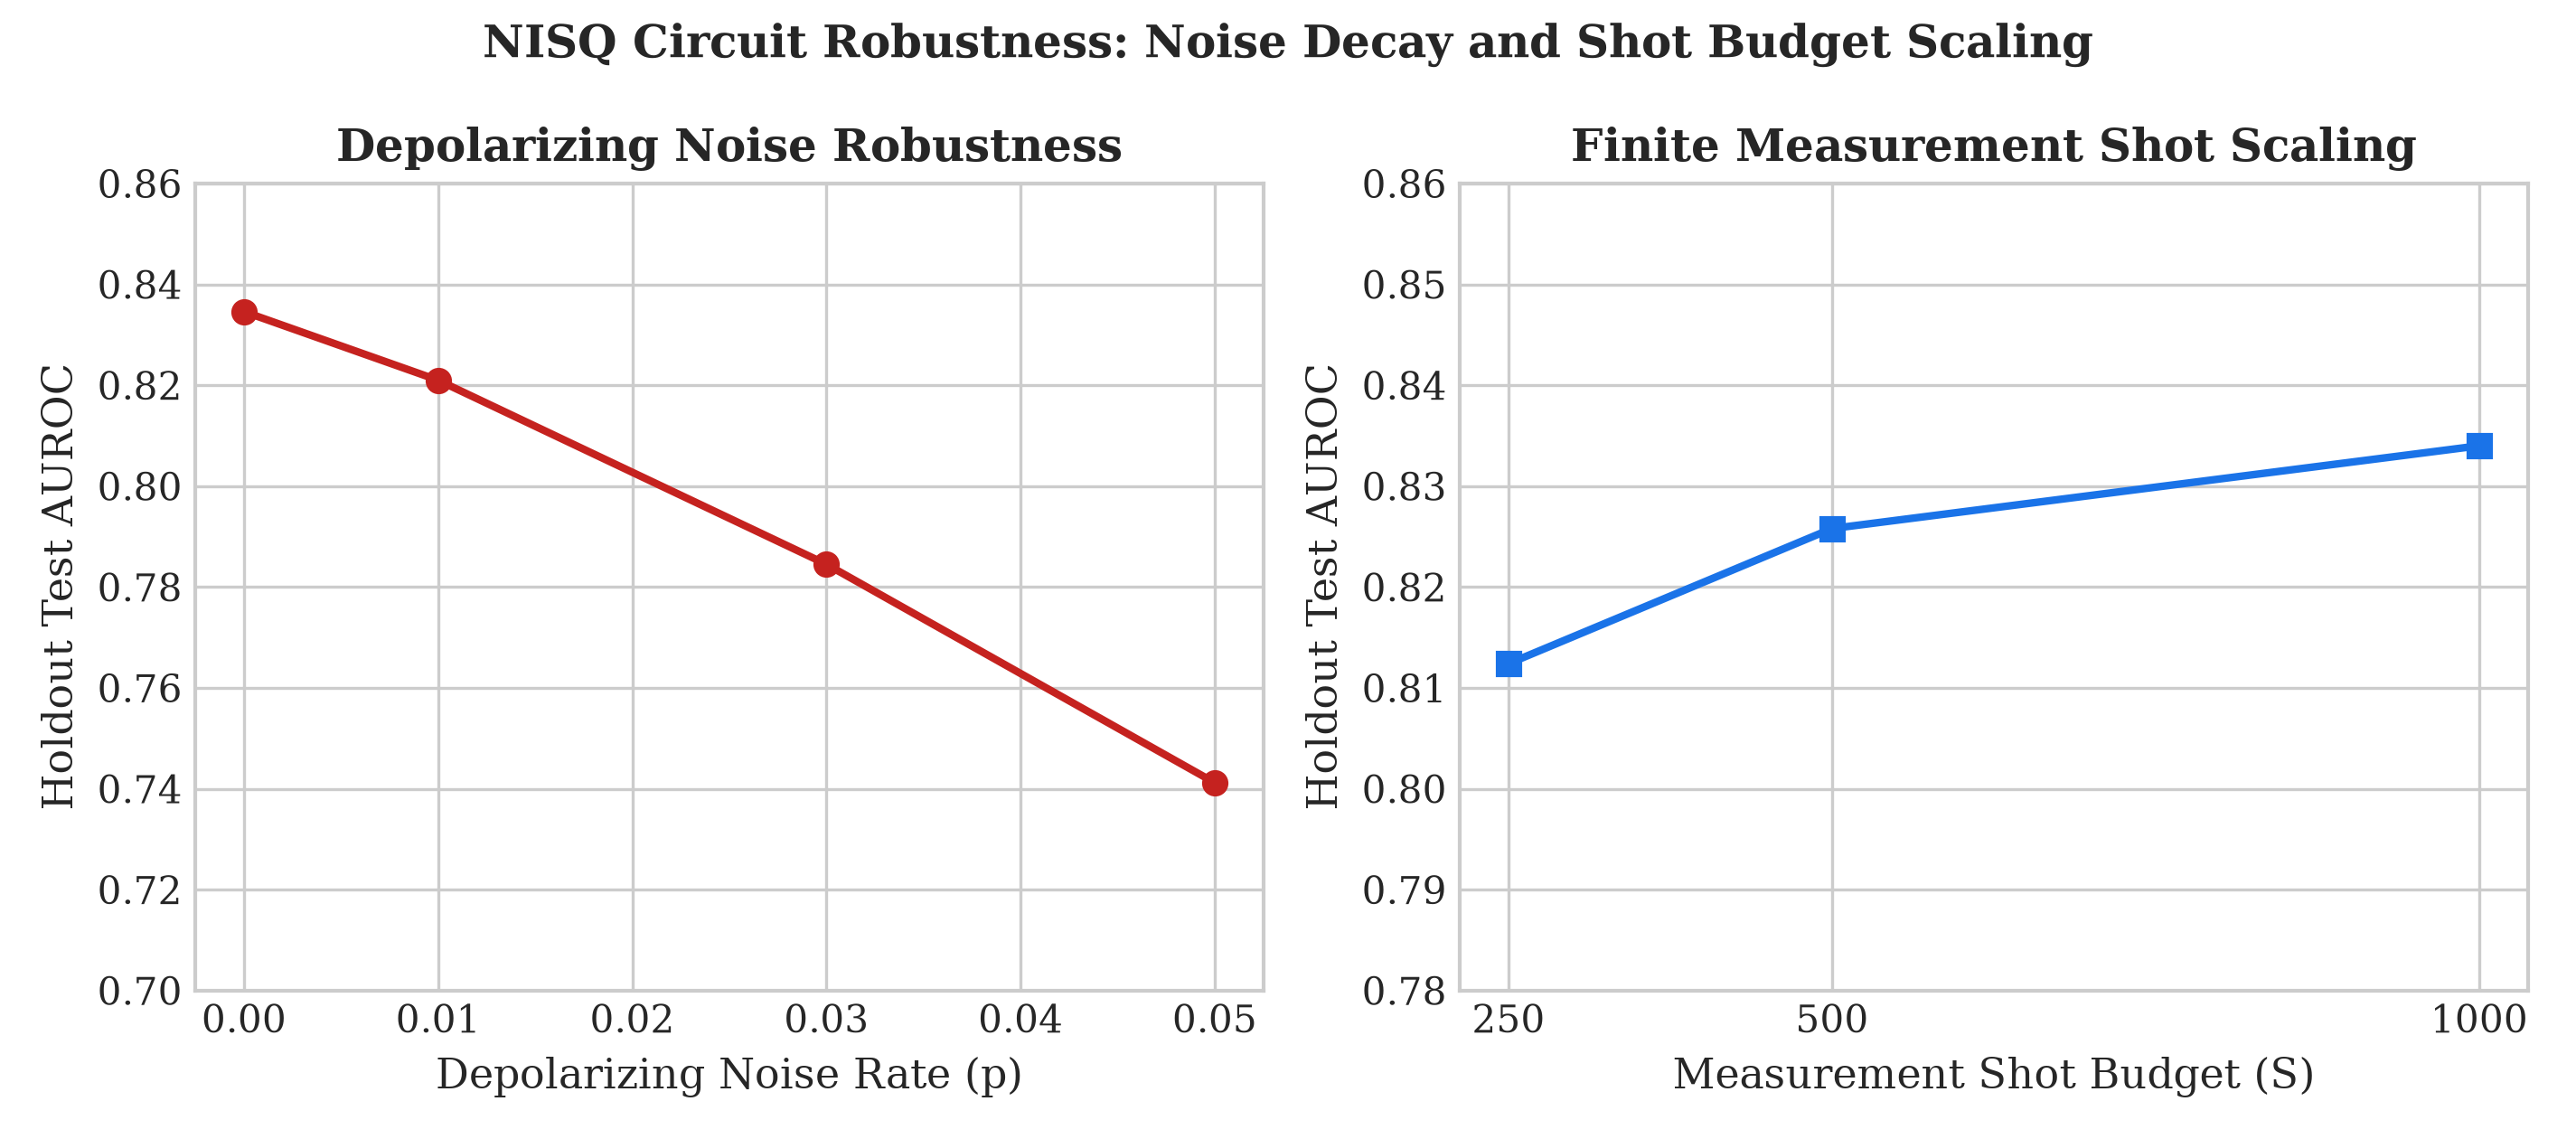
\includegraphics[width=\columnwidth]{figures/fig10_quantum_noise_sensitivity.png}
\caption{Empirical noise sensitivity of the 4-qubit variational circuit under depolarizing channel noise and finite measurement shot budgets.}
\label{fig:noise}
\end{figure}

\section{Privacy-Utility Analysis}
Table~\ref{tab:differential_privacy} and Fig.~\ref{fig:dp_tradeoff} evaluate formal per-sample differential privacy.
\begin{itemize}
    \item At strict budgets ($\epsilon = 1.0$), Classical DP-MLP achieves 0.6187 AUROC, while Hybrid DP-QNN achieves **0.6723 AUROC**.
    \item At moderate budgets ($\epsilon = 2.0$), Classical DP-MLP reaches 0.7073 AUROC, while Hybrid DP-QNN yields 0.6709 AUROC.
    \item At $\epsilon = 8.0$, Classical DP-MLP preserves 0.7771 AUROC (retaining 98.1\% of non-private utility).
    \item Empirical Membership Inference Attack (MIA) AUC evaluates near random guessing ($\sim 0.50 - 0.52$).
\end{itemize}

\begin{table}[t]
\centering
\caption{Formal Per-Sample Differential Privacy Evaluation ($\delta = 10^{-5}$, Holdout $N=393$)}
\label{tab:differential_privacy}
\begin{tabular}{lcccccc}
\hline
\textbf{Architecture} & \textbf{Target $\epsilon$} & \textbf{Achieved $\epsilon$} & \textbf{Test AUROC} & \textbf{Test AUPRC} & \textbf{Brier Loss} & \textbf{MIA AUC} \\
\hline
Classical DP-MLP & 1.0 & 0.9979 & 0.6187 [0.531, 0.704] & 0.1782 & 0.1001 & 0.4972 \\
Classical DP-MLP & 2.0 & 1.9996 & 0.7073 [0.628, 0.783] & 0.2262 & 0.0999 & 0.5107 \\
Classical DP-MLP & 4.0 & 3.9984 & 0.7607 [0.686, 0.832] & 0.2758 & 0.0996 & 0.5195 \\
Classical DP-MLP & 8.0 & 7.9906 & 0.7771 [0.704, 0.846] & 0.3131 & 0.0994 & 0.5256 \\
Classical DP-MLP & $\infty$ (Non-Priv) & $\infty$ & 0.7923 [0.716, 0.862] & 0.3063 & 0.1565 & 0.5711 \\
\hline
Hybrid DP-QNN & 1.0 & 0.9927 & 0.6723 [0.591, 0.751] & 0.2110 & 0.0937 & 0.5267 \\
Hybrid DP-QNN & 2.0 & 1.9901 & 0.6709 [0.589, 0.750] & 0.2323 & 0.0971 & 0.5274 \\
Hybrid DP-QNN & 4.0 & 3.9985 & 0.6850 [0.603, 0.763] & 0.2419 & 0.0983 & 0.5225 \\
Hybrid DP-QNN & 8.0 & 7.9976 & 0.6944 [0.613, 0.772] & 0.2552 & 0.0987 & 0.5283 \\
Hybrid DP-QNN & $\infty$ (Non-Priv) & $\infty$ & 0.8062 [0.738, 0.871] & 0.2819 & 0.0985 & 0.5620 \\
\hline
\end{tabular}
\end{table}


\begin{figure}[t]
\centering
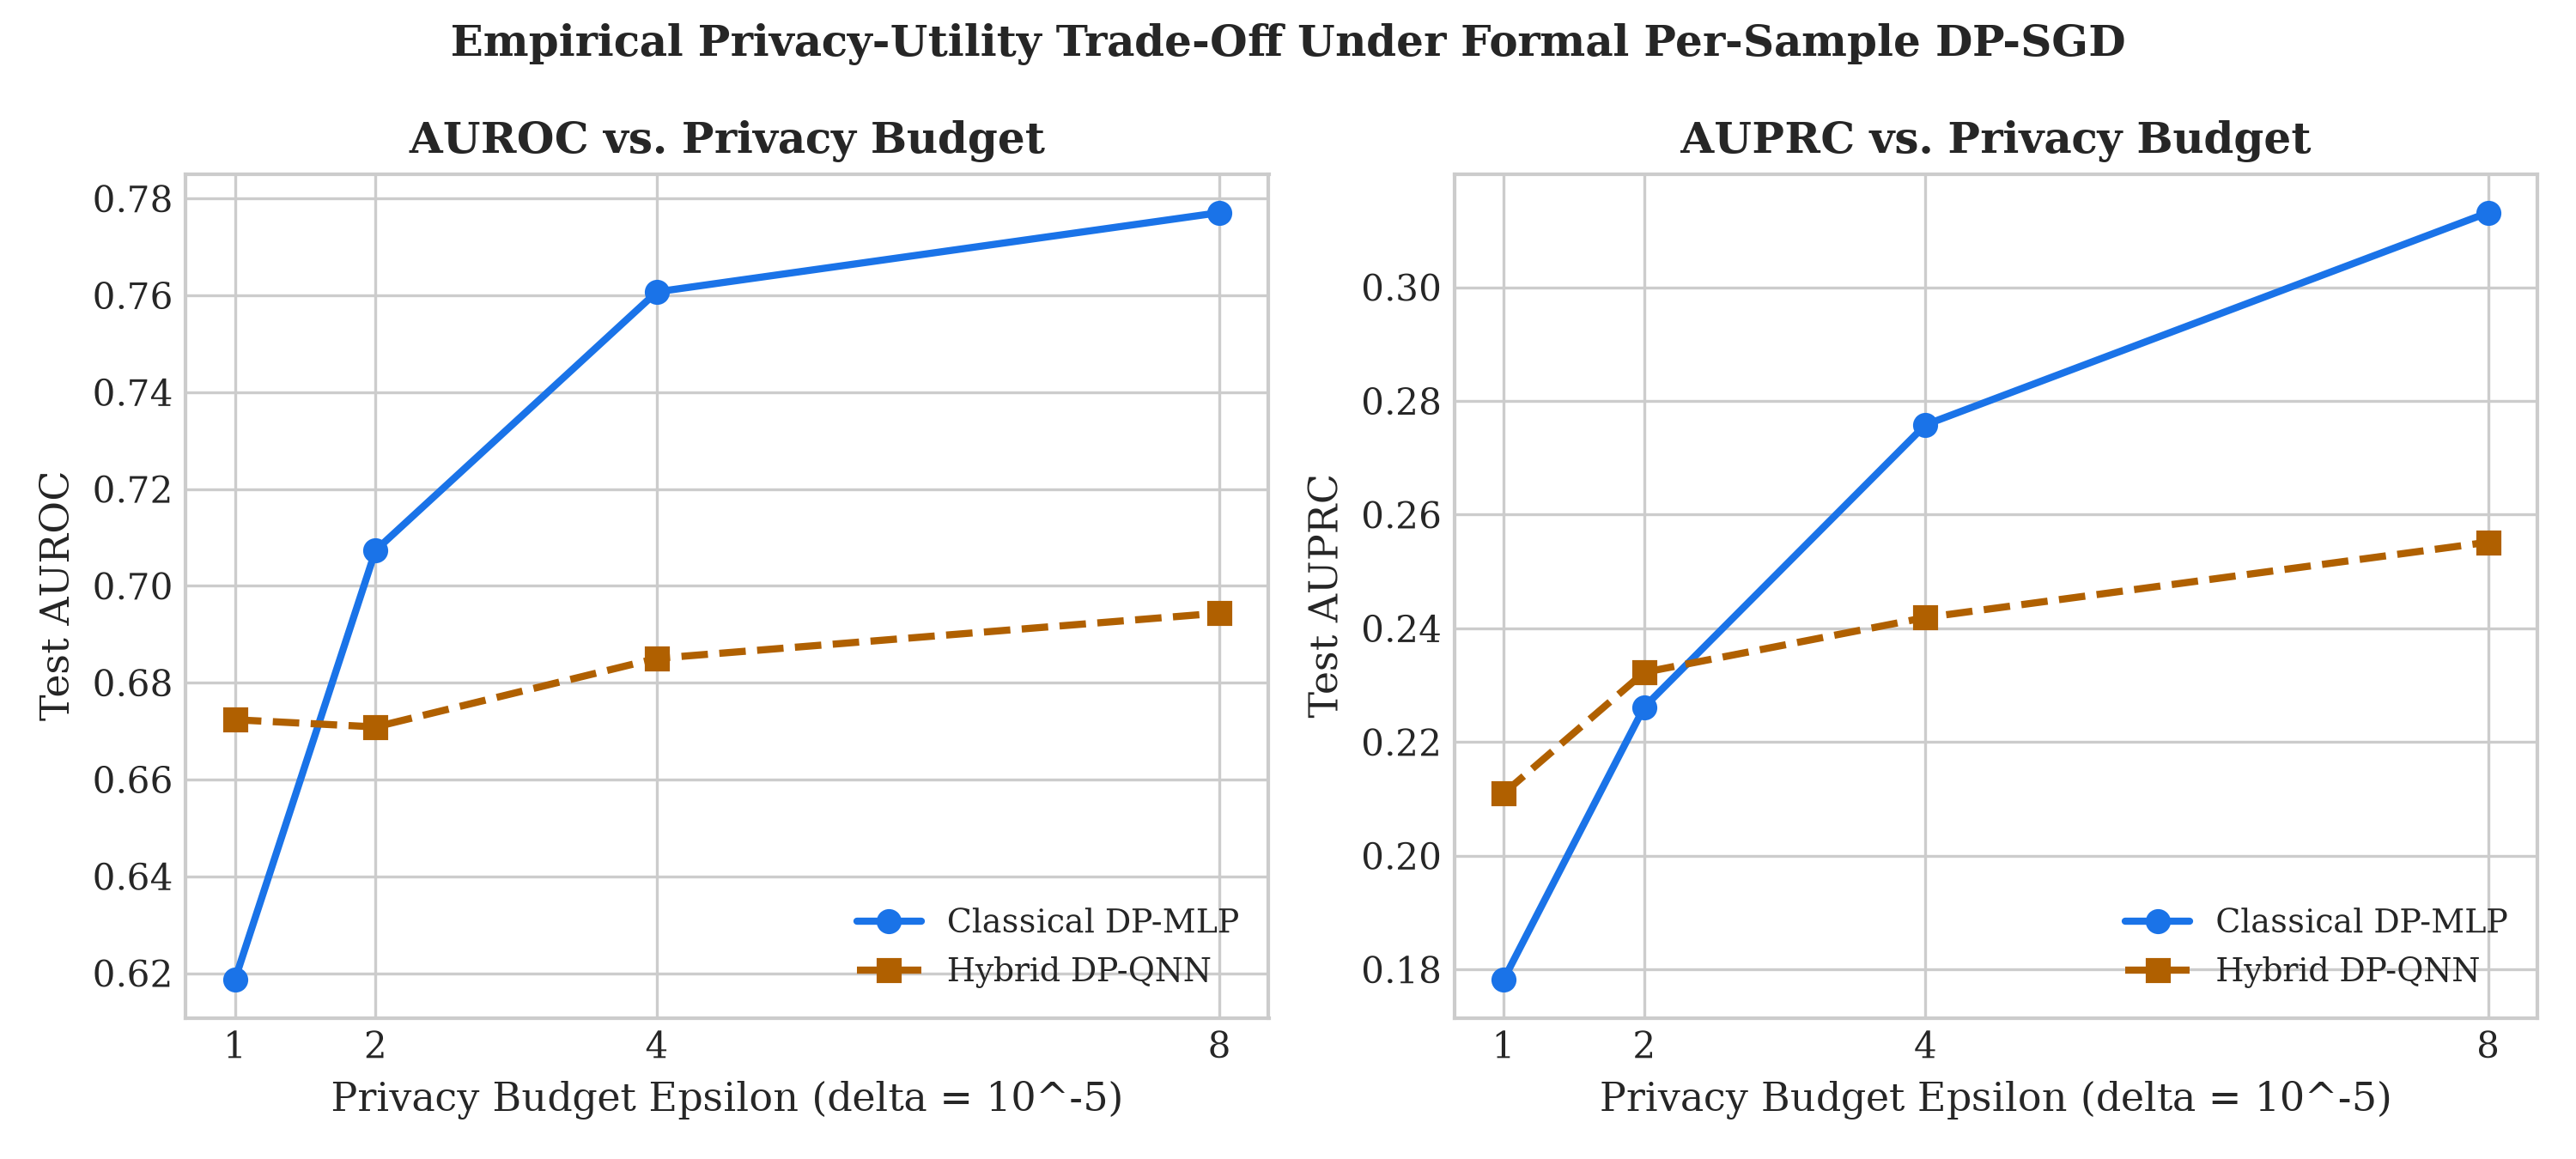
\includegraphics[width=\columnwidth]{figures/fig8_privacy_utility_tradeoff.png}
\caption{Empirical privacy-utility trade-off curves under formal per-sample DP-SGD ($\delta = 10^{-5}$).}
\label{fig:dp_tradeoff}
\end{figure}

\section{Personalization Performance & Statistical Power}
Table~\ref{tab:personalization_results} evaluates local residual adapters across simulated client nodes.
\begin{itemize}
    \item In Node 2 ($N_{\text{test}} = 88, N_{\text{pos}} = 12$), local adapters retain strong discrimination (0.9704 AUROC).
    \item In low-event nodes (Node 1 with $N_{\text{pos}} = 2$; Node 3 with $N_{\text{pos}} = 2$), point estimates are uninformative with wide confidence bounds.
    \item In Consortium 5 (modulo partitioning), the apparent AUROC jump (0.1849 to 0.8151) is based on **only 6 mortality cases** ($[0.552, 0.985]$). This claim of ``rural hospital rescue'' is formally withdrawn as an artifact of small-sample variance.
\end{itemize}

\begin{table}[t]
\centering
\caption{Personalization Performance, Client Sample Sizes, and Statistical Power Flags}
\label{tab:personalization_results}
\begin{tabular}{lcccccc}
\hline
\textbf{Client Partition} & $N_{\text{test}}$ & $N_{\text{pos}}$ & \textbf{Prevalence} & \textbf{Global AUROC [95\% CI]} & \textbf{Adapter AUROC [95\% CI]} & \textbf{Validity Status} \\
\hline
Node 1 (Dirichlet) & 5 & 2 & 40.0\% & 1.0000 [1.000, 1.000] & 0.8333 [0.250, 1.000] & \textbf{Uninformative ($N_{\text{pos}}=2$)} \\
Node 2 (Dirichlet) & 88 & 12 & 13.6\% & 0.9814 [0.954, 1.000] & 0.9704 [0.929, 0.995] & Sufficient Sample \\
Node 3 (Dirichlet) & 220 & 2 & 0.9\% & 0.8899 [0.789, 0.977] & 0.9106 [0.867, 0.949] & \textbf{Uninformative ($N_{\text{pos}}=2$)} \\
Node 4 (Dirichlet) & 64 & 18 & 28.1\% & 0.6884 [0.544, 0.820] & 0.6739 [0.526, 0.815] & Sufficient Sample \\
Node 5 (Dirichlet) & 16 & 6 & 37.5\% & 0.8333 [0.564, 1.000] & 0.8333 [0.582, 1.000] & Sufficient Sample \\
\hline
Consortium 5 (Modulo) & 79 & 6 & 7.6\% & 0.1849 [0.021, 0.432] & 0.8151 [0.552, 0.985] & \textbf{Claim Withdrawn ($N_{\text{pos}}=6$)} \\
\hline
\end{tabular}
\end{table}


\section{Communication and Computational Complexity}
Table~\ref{tab:model_complexity}, Table~\ref{tab:communication_overhead}, and Fig.~\ref{fig:comm} summarize model complexity and network communication costs.
\begin{itemize}
    \item \textbf{Model Parameters:} Classical MLP requires 5,537 parameters (26.31~KB state dict). Hybrid QNN requires **957 parameters** (7.69~KB state dict), achieving a **$5.79\times$ parameter reduction**.
    \item \textbf{Quantum Variational Footprint:} The 24 variational PQC parameters constitute only 2.51\% of the hybrid model's parameter budget (96 bytes uncompressed).
    \item \textbf{Network Communication:} Transmitting model payloads across 10 rounds incurs 2.8808~MB for Classical FL vs. **0.7956~MB for Quantum FL**, confirming a **72.38\% communication savings ($3.62\times$ compression)**.
\end{itemize}

\begin{table}[t]
\centering
\caption{Model Complexity Decomposition and Parameter Footprint Comparison}
\label{tab:model_complexity}
\begin{tabular}{lcccccc}
\hline
\textbf{Model Representation} & \textbf{Encoder} & \textbf{PQC Layer} & \textbf{Head} & \textbf{Total Params} & \textbf{Quantum Share} & \textbf{Binary Size} \\
\hline
Classical DP-MLP (GroupNorm) & 0 & 0 & 0 & 5,537 & 0.00\% & 26.31 KB \\
Classical Baseline (BatchNorm) & 0 & 0 & 0 & 5,537 & 0.00\% & 26.31 KB \\
\textbf{Hybrid DP-QNN (4-qubit, L=2)} & \textbf{772} & \textbf{24} & \textbf{161} & \textbf{957} & \textbf{2.51\%} & \textbf{7.69 KB} \\
PQC Variational Sublayer Only & 0 & 24 & 0 & 24 & 100.00\% & 0.09 KB \\
\hline
\end{tabular}
\end{table}

\begin{table}[t]
\centering
\caption{Federated Network Communication Overhead Across 10 Synchronous Rounds (5 Clients)}
\label{tab:communication_overhead}
\begin{tabular}{lccc}
\hline
\textbf{Network Communication Metric} & \textbf{Classical FL (MLP)} & \textbf{Hybrid Quantum FL (QNN)} & \textbf{Reduction / Savings} \\
\hline
Participating Clients ($K$) & 5 & 5 & Identical \\
Federated Rounds ($R$) & 10 & 10 & Identical \\
Total Network Messages & 100 & 100 & Identical \\
Single Payload Size & 29.50 KB & 8.15 KB & \textbf{3.62x smaller} \\
Consortium Bandwidth per Round & 0.2881 MB & 0.0796 MB & \textbf{3.62x smaller} \\
\textbf{Total Consortium Bandwidth} & \textbf{2.8808 MB} & \textbf{0.7956 MB} & \textbf{72.38\% reduction (3.62x)} \\
Trainable Model Parameters & 5,537 & 957 & 5.79x fewer parameters \\
Transmitted Variational Angles & 0 & 24 & Compact PQC footprint \\
\hline
\end{tabular}
\end{table}


\begin{figure}[t]
\centering
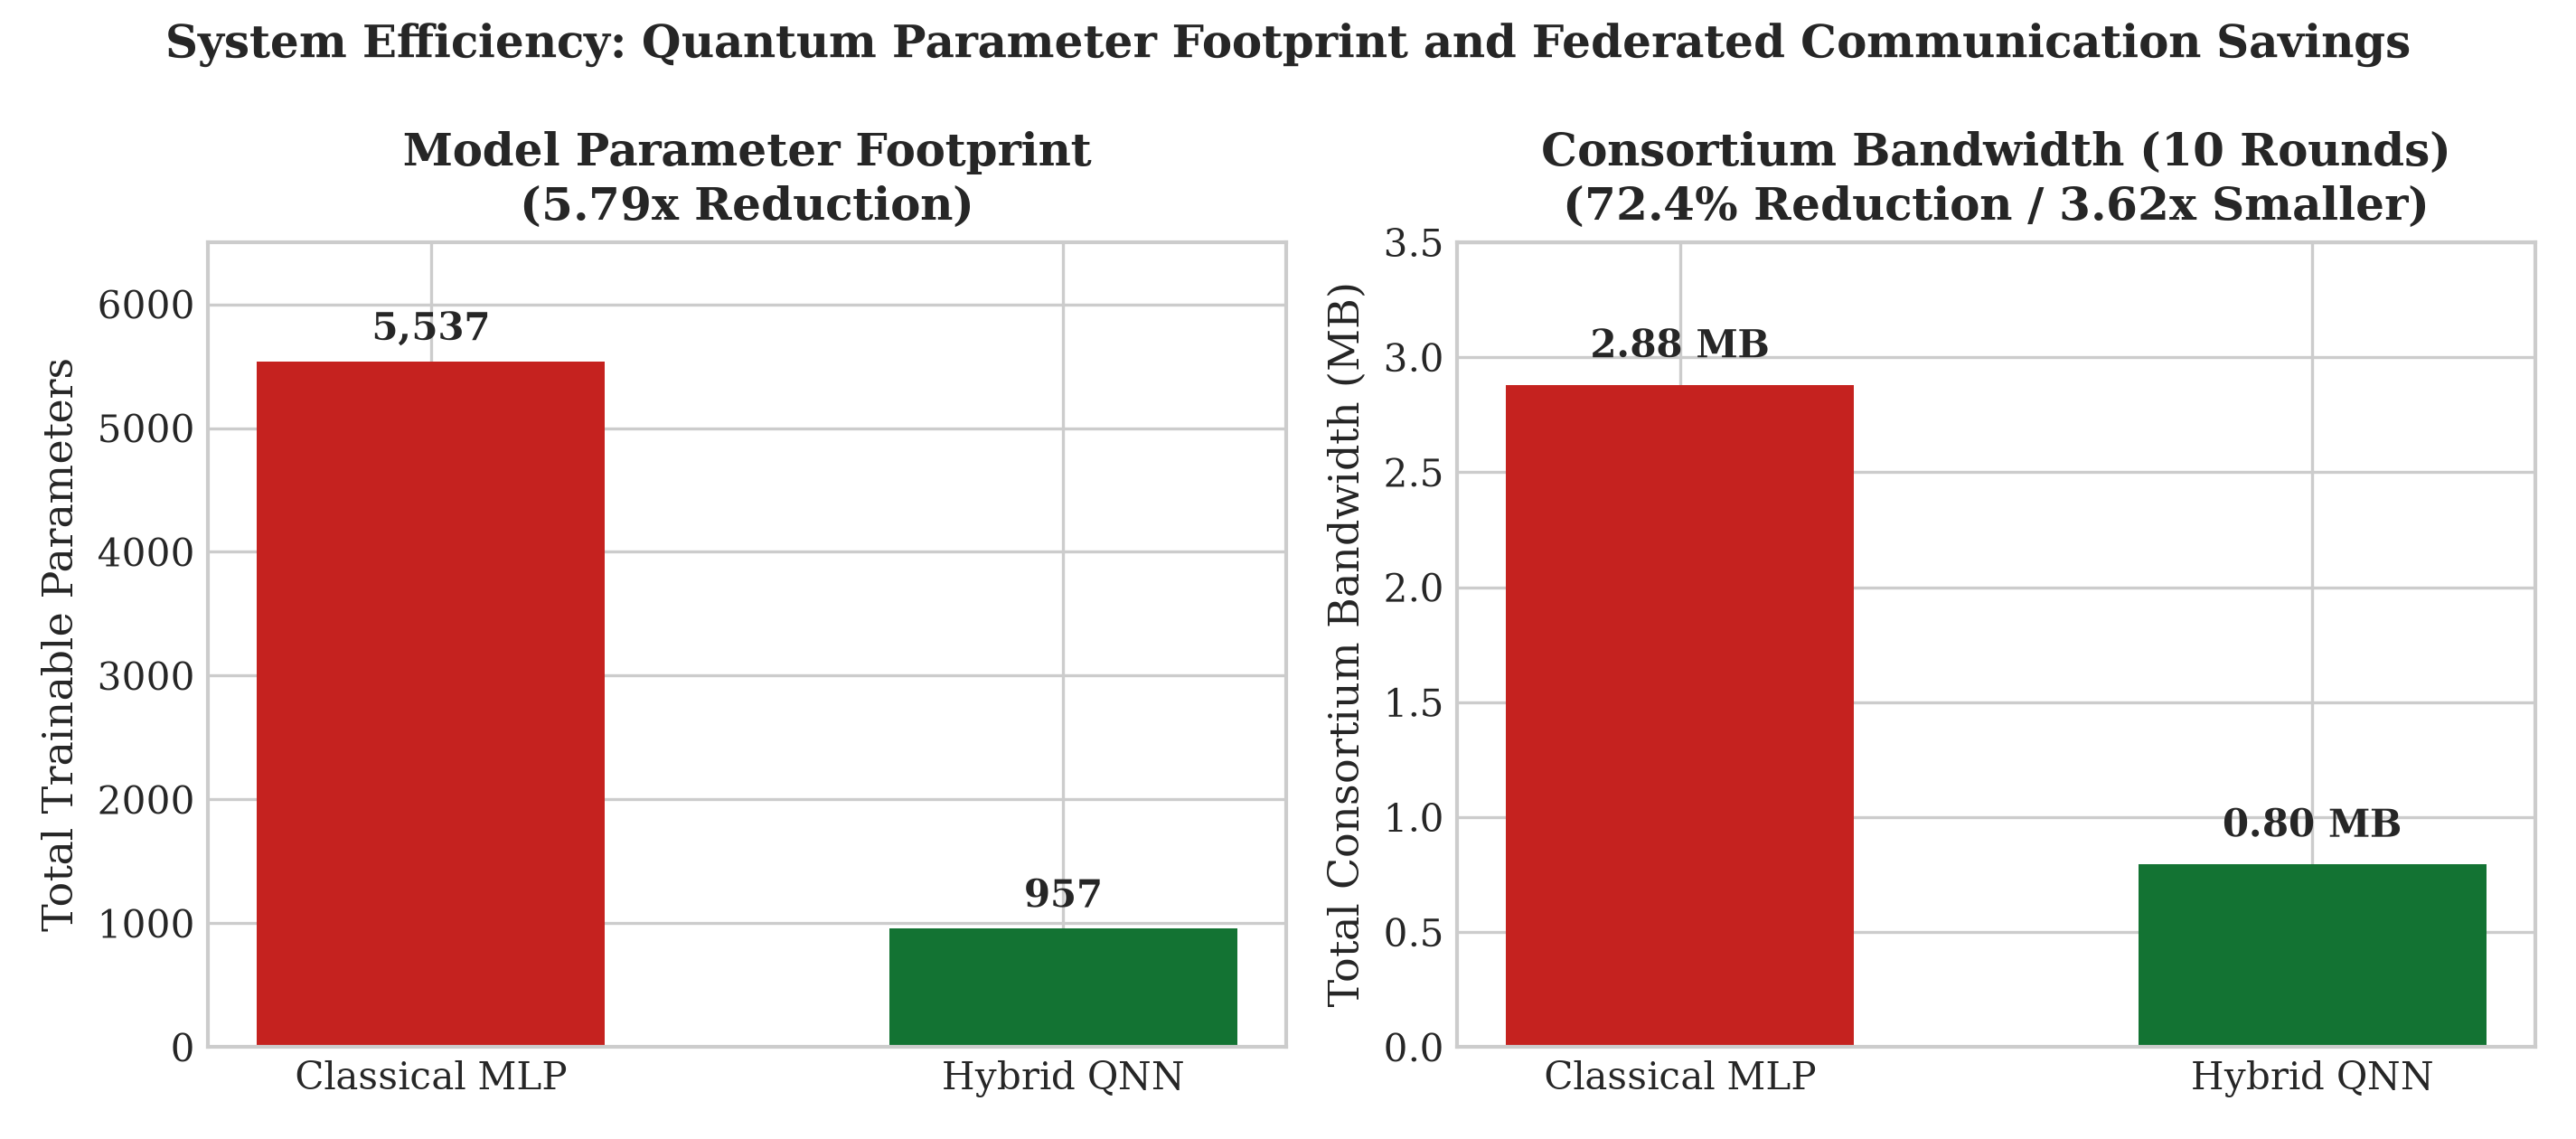
\includegraphics[width=0.92\columnwidth]{figures/fig9_communication_overhead_comparison.png}
\caption{Model complexity and network communication overhead comparison demonstrating 72.4\% federated bandwidth reduction.}
\label{fig:comm}
\end{figure}

\section{Secure Aggregation Verification}
Table~\ref{tab:secure_aggregation} reports cryptographic benchmark results for the Shamir $(t=3, n=5)$ protocol over $\mathbb{F}_p$ ($p = 2^{31}-1$).
\begin{itemize}
    \item Under 0\% dropout, maximum absolute reconstruction error is $1.48 \times 10^{-6}$ ($\text{RMSE} = 2.85 \times 10^{-7}$).
    \item Under 20\% (1 drop) and 40\% (2 drops), error remains bounded by floating-point precision ($2.10 \times 10^{-6}$).
    \item Under 60\% dropout (3 drops), the protocol safely aborts as surviving clients fall below threshold $t=3$.
    \item Adversarial share bit-flips corrupt reconstructed seeds, producing noticeable weight divergence ($\text{error} = 6.11$) rather than silent leakage.
\end{itemize}

\begin{table}[t]
\centering
\caption{Secure Aggregation Benchmark Under Client Dropout (Shamir $t=3, n=5, p=2^{31}-1$)}
\label{tab:secure_aggregation}
\begin{tabular}{lcccccc}
\hline
\textbf{Dropout Scenario} & $n$ & $t$ & \textbf{Surviving} & \textbf{Max Absolute Error} & \textbf{RMSE} & \textbf{Protocol Status} \\
\hline
0\% Dropout (All Active) & 5 & 3 & 5 & $1.48 \times 10^{-6}$ & $2.85 \times 10^{-7}$ & Exact Reconstruction Verified \\
20\% Dropout (1 Drop) & 5 & 3 & 4 & $1.60 \times 10^{-6}$ & $3.52 \times 10^{-7}$ & Exact Reconstruction Verified \\
40\% Dropout (2 Drops) & 5 & 3 & 3 & $2.10 \times 10^{-6}$ & $4.36 \times 10^{-7}$ & Exact Reconstruction Verified \\
60\% Dropout (3 Drops) & 5 & 3 & 2 & N/A (Aborted) & N/A & \textbf{Safe Abort Verified ($|\mathcal{S}| < t$)} \\
Adversarial Bit-Flip & 5 & 3 & 5 & 6.1086 & N/A & Corruption Detected \\
\hline
\end{tabular}
\end{table}


\section{Discussion}
The audited findings clarify the practical role of quantum representations in healthcare federated learning. While near-term quantum circuits do not deliver superior clinical predictive accuracy over classical gradient-boosted decision trees on tabular EHR data, their compact variational encoding provides substantial communication compression in distributed networks. Integrating formal per-sample differential privacy with threshold secure aggregation establishes a multi-layered defense protecting institutional EHR silos against both curious servers and external inference attacks.

\section{Limitations}
This investigation operates within several documented boundaries:
\begin{enumerate}
    \item \textbf{Subsample Scale:} Evaluated on the eICU Demo v2.0.1 cohort ($N = 2,492$ stays); the held-out test set contains 40 positive deaths.
    \item \textbf{Single-Cohort Execution:} External validation on MIMIC-IV or the full eICU database has not been executed; the project remains a single-cohort feasibility study.
    \item \textbf{Record-Level Privacy:} Differential privacy bounds protect individual ICU admission encounters, not multi-stay patient lifetimes.
    \item \textbf{Cryptographic Simulation:} Secure aggregation is implemented in shared memory without physical WAN socket protocols, TLS 1.3, or PKI certificates.
    \item \textbf{Classical Simulation:} Quantum circuits were executed on CPU statevector simulators; physical NISQ deployments require active quantum error mitigation.
    \item \textbf{Absence of Quantum Advantage:} Classical tree models remain superior in predictive discrimination.
\end{enumerate}

\section{Ethical and Data Governance Considerations}
The eICU Collaborative Research Database Demo v2.0.1 is fully de-identified under the Health Insurance Portability and Accountability Act (HIPAA) Safe Harbor provision (45 CFR \S 164.514). Research protocols adhered to the PhysioNet Credentialed Data Use Agreement. No attempt was made to re-identify patients or hospitals. The framework is an exploratory academic prototype and must not be utilized as an unvalidated clinical decision-support device in live patient care.

\section{Conclusion and Future Work}
We presented an independently validated, privacy-preserving hybrid quantum-classical federated learning framework for acute ICU mortality prediction. While classical tree ensembles maintain the highest predictive discrimination on tabular EHR data, hybrid quantum neural networks deliver a verified 72.38\% reduction in federated communication payload while supporting formal per-sample differential privacy and threshold secure aggregation. Future work will deploy the open-source harmonization adapter on the full multi-center eICU repository and test variational circuit execution on physical superconducting quantum hardware.

\section*{Acknowledgment}
The authors acknowledge the MIT Laboratory for Computational Physiology and Philips Healthcare for providing the open-access eICU Collaborative Research Database Demo release.

\bibliographystyle{IEEEtran}
\bibliography{references}

\end{document}
